\section{Results}
\label{results}
By using the approach described in the previous section, the new mapper grew
capable of providing critical features for medical and scientific computing.
This section describes each of these features in sufficient detail in the
following text.

\newcommand{\ignore}[1]{}

\subsection{Stochastic Jittering}
Because ray-casting effectively samples a discrete signal (voxel values along
the ray trajectory), the distance between those sampling points heavily
influences how accurately the volume data is represented.  Due to well
established limitations described by the sampling theorem, low sampling rates
may result in aliasing effects often referred to as wood-grain artifacts
as shown in ~\Autoref{fig:jittering_without} in the context of volume rendering
\ignore{~\citep{RTVG_jittering}}. Reducing the distance between samples
neutralizes these artifacts but takes an important toll on performance.

The mapper supports stochastic jittering, which is an alternative technique to
counteract wood-grain artifacts by adding a random offset to the rays in the
viewing direction thereby breaking the coherence between neighboring fragments
which causes the aliased patterns become apparent
as shown in ~\Autoref{fig:jittering_with}.  Jittering is implemented by creating a
random noise texture (using \texttt{vtkPerlinNoise}) and applying the offset to
the ray's starting point, thus has a much lower performance penalty than
reducing the sampling distance.

\begin{figure}[htb]
\centering
  \begin{subfigure}[b]{.5\columnwidth}
    \centering
    \includegraphics[width=\textwidth]{cactus_holland_woodgrain.png}
    \caption{Wood-grain artifacts.}
    \label{fig:jittering_without}
  \end{subfigure}%
  \begin{subfigure}[b]{.5\columnwidth}
    \centering
    \includegraphics[width=\textwidth]{cactus_holland_jittering.png}
    \caption{With jittering enabled.}
    \label{fig:jittering_with}
  \end{subfigure}
  \caption{Stochastic jittering.}
  \label{fig:jittering}
\end{figure}

\subsection{Clipping}
\label{clipping}
A set of infinite planes can be defined to clip the volume to reveal inner
detail, as shown in Figure 4.  The visibility of each sample along the ray
is determined by computing the sample's distance to each plane and testing
for it being in front or behind.

The current implementation iterates through each of the planes before entering
the ray marching loop in order to early-discard rays which fall in any of the
following criteria:

\begin{enumerate}
\item Entering the volume on the clipped side and exiting before ever
	intersecting the plane (the ray only traverses clipped space).
\item Intersecting overlapping geometry before the plane (z-buffer compositing).
\end{enumerate}

\subsection{Cropping} Cropping refers to 27 regions that defined by two
planes along each coordinate axis of the volume and can be independently turned
on (visible) or off (invisible) to produce a variety of different cropping
effects, as shown in ~\Autoref{fig:cropping}. Cropping is implemented by
determining the cropping region of each sample location along the ray and
including only those samples that fall within a visible region.

\begin{figure}[htb]
  \centering
  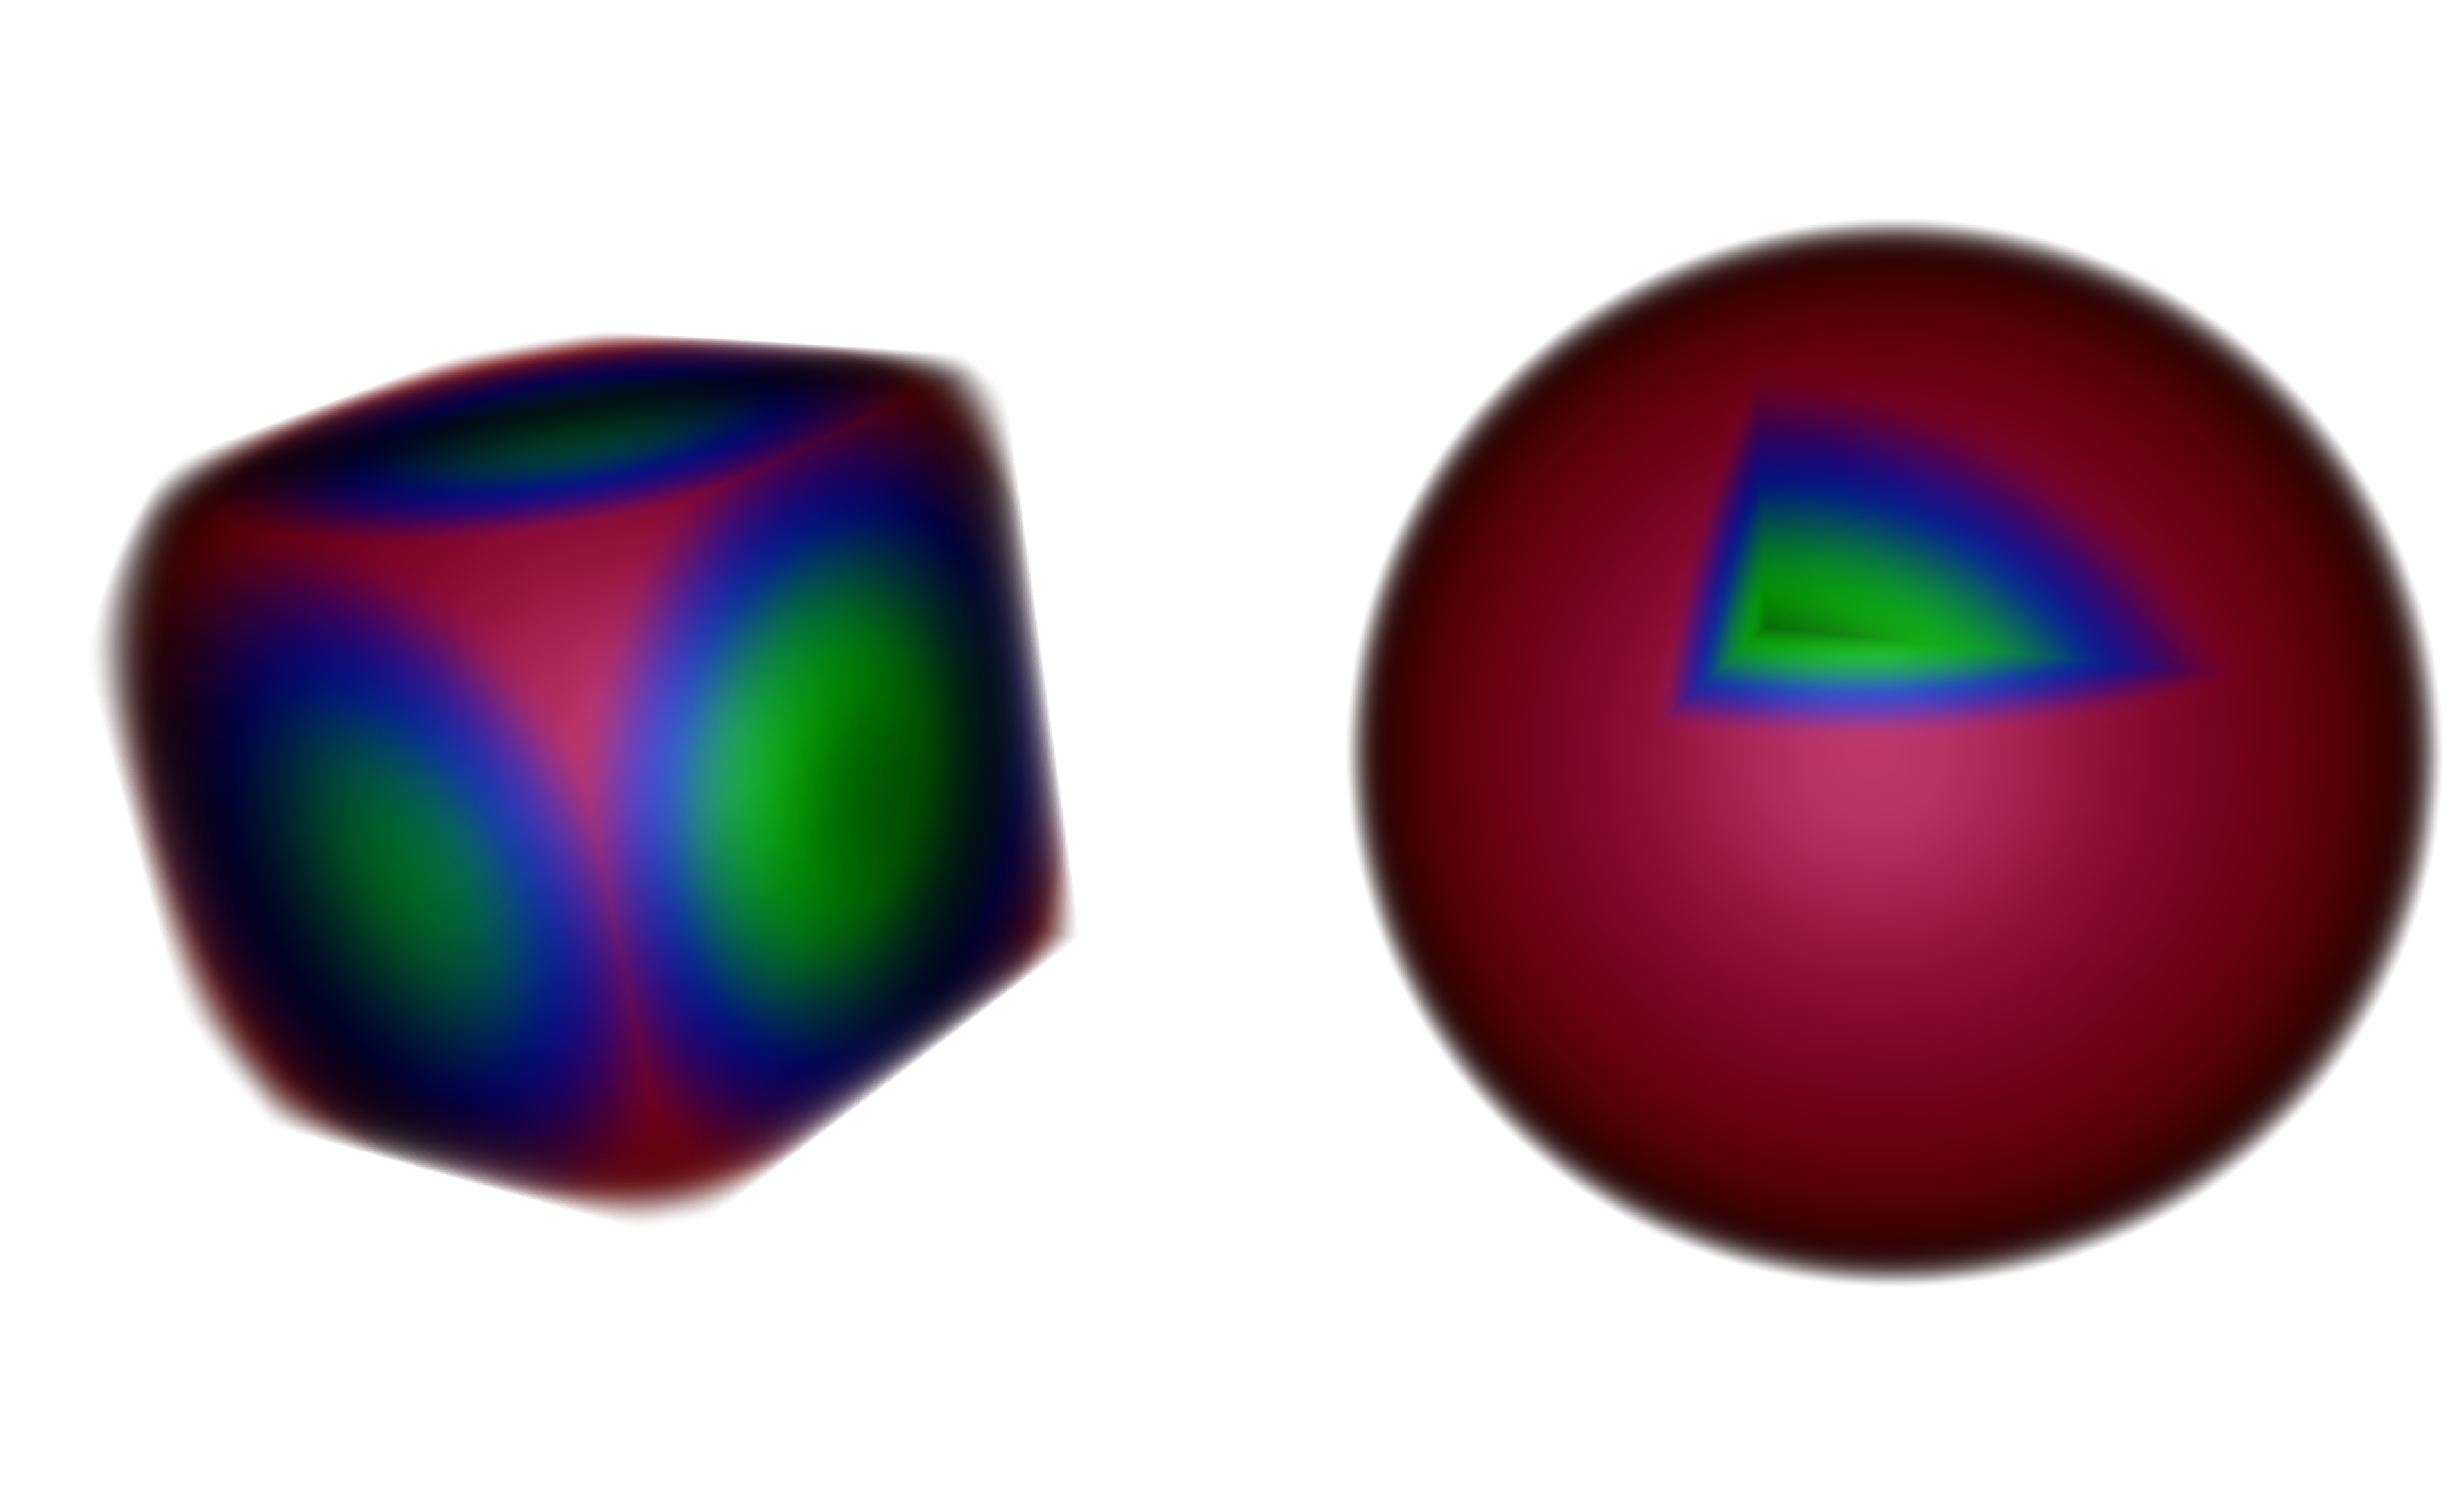
\includegraphics[width=2.5in]{SphereCropping.png}
  \caption{A sphere is cropped using two different configurations of cropping regions.}
  \label{fig:cropping}
\end{figure}

\subsection{Wide Support of Data Types}
The mapper supports most signed and unsigned data types such as short, int,
float and double as well as the two most common data abstractions in VTK,
cell and point data.  Bias and scale factors are pre-computed and passed into
the fragment shader to normalize the data values for correct look-up table
mapping.

\begin{figure}[htb]
  \centering
  \begin{subfigure}[b]{\columnwidth}
    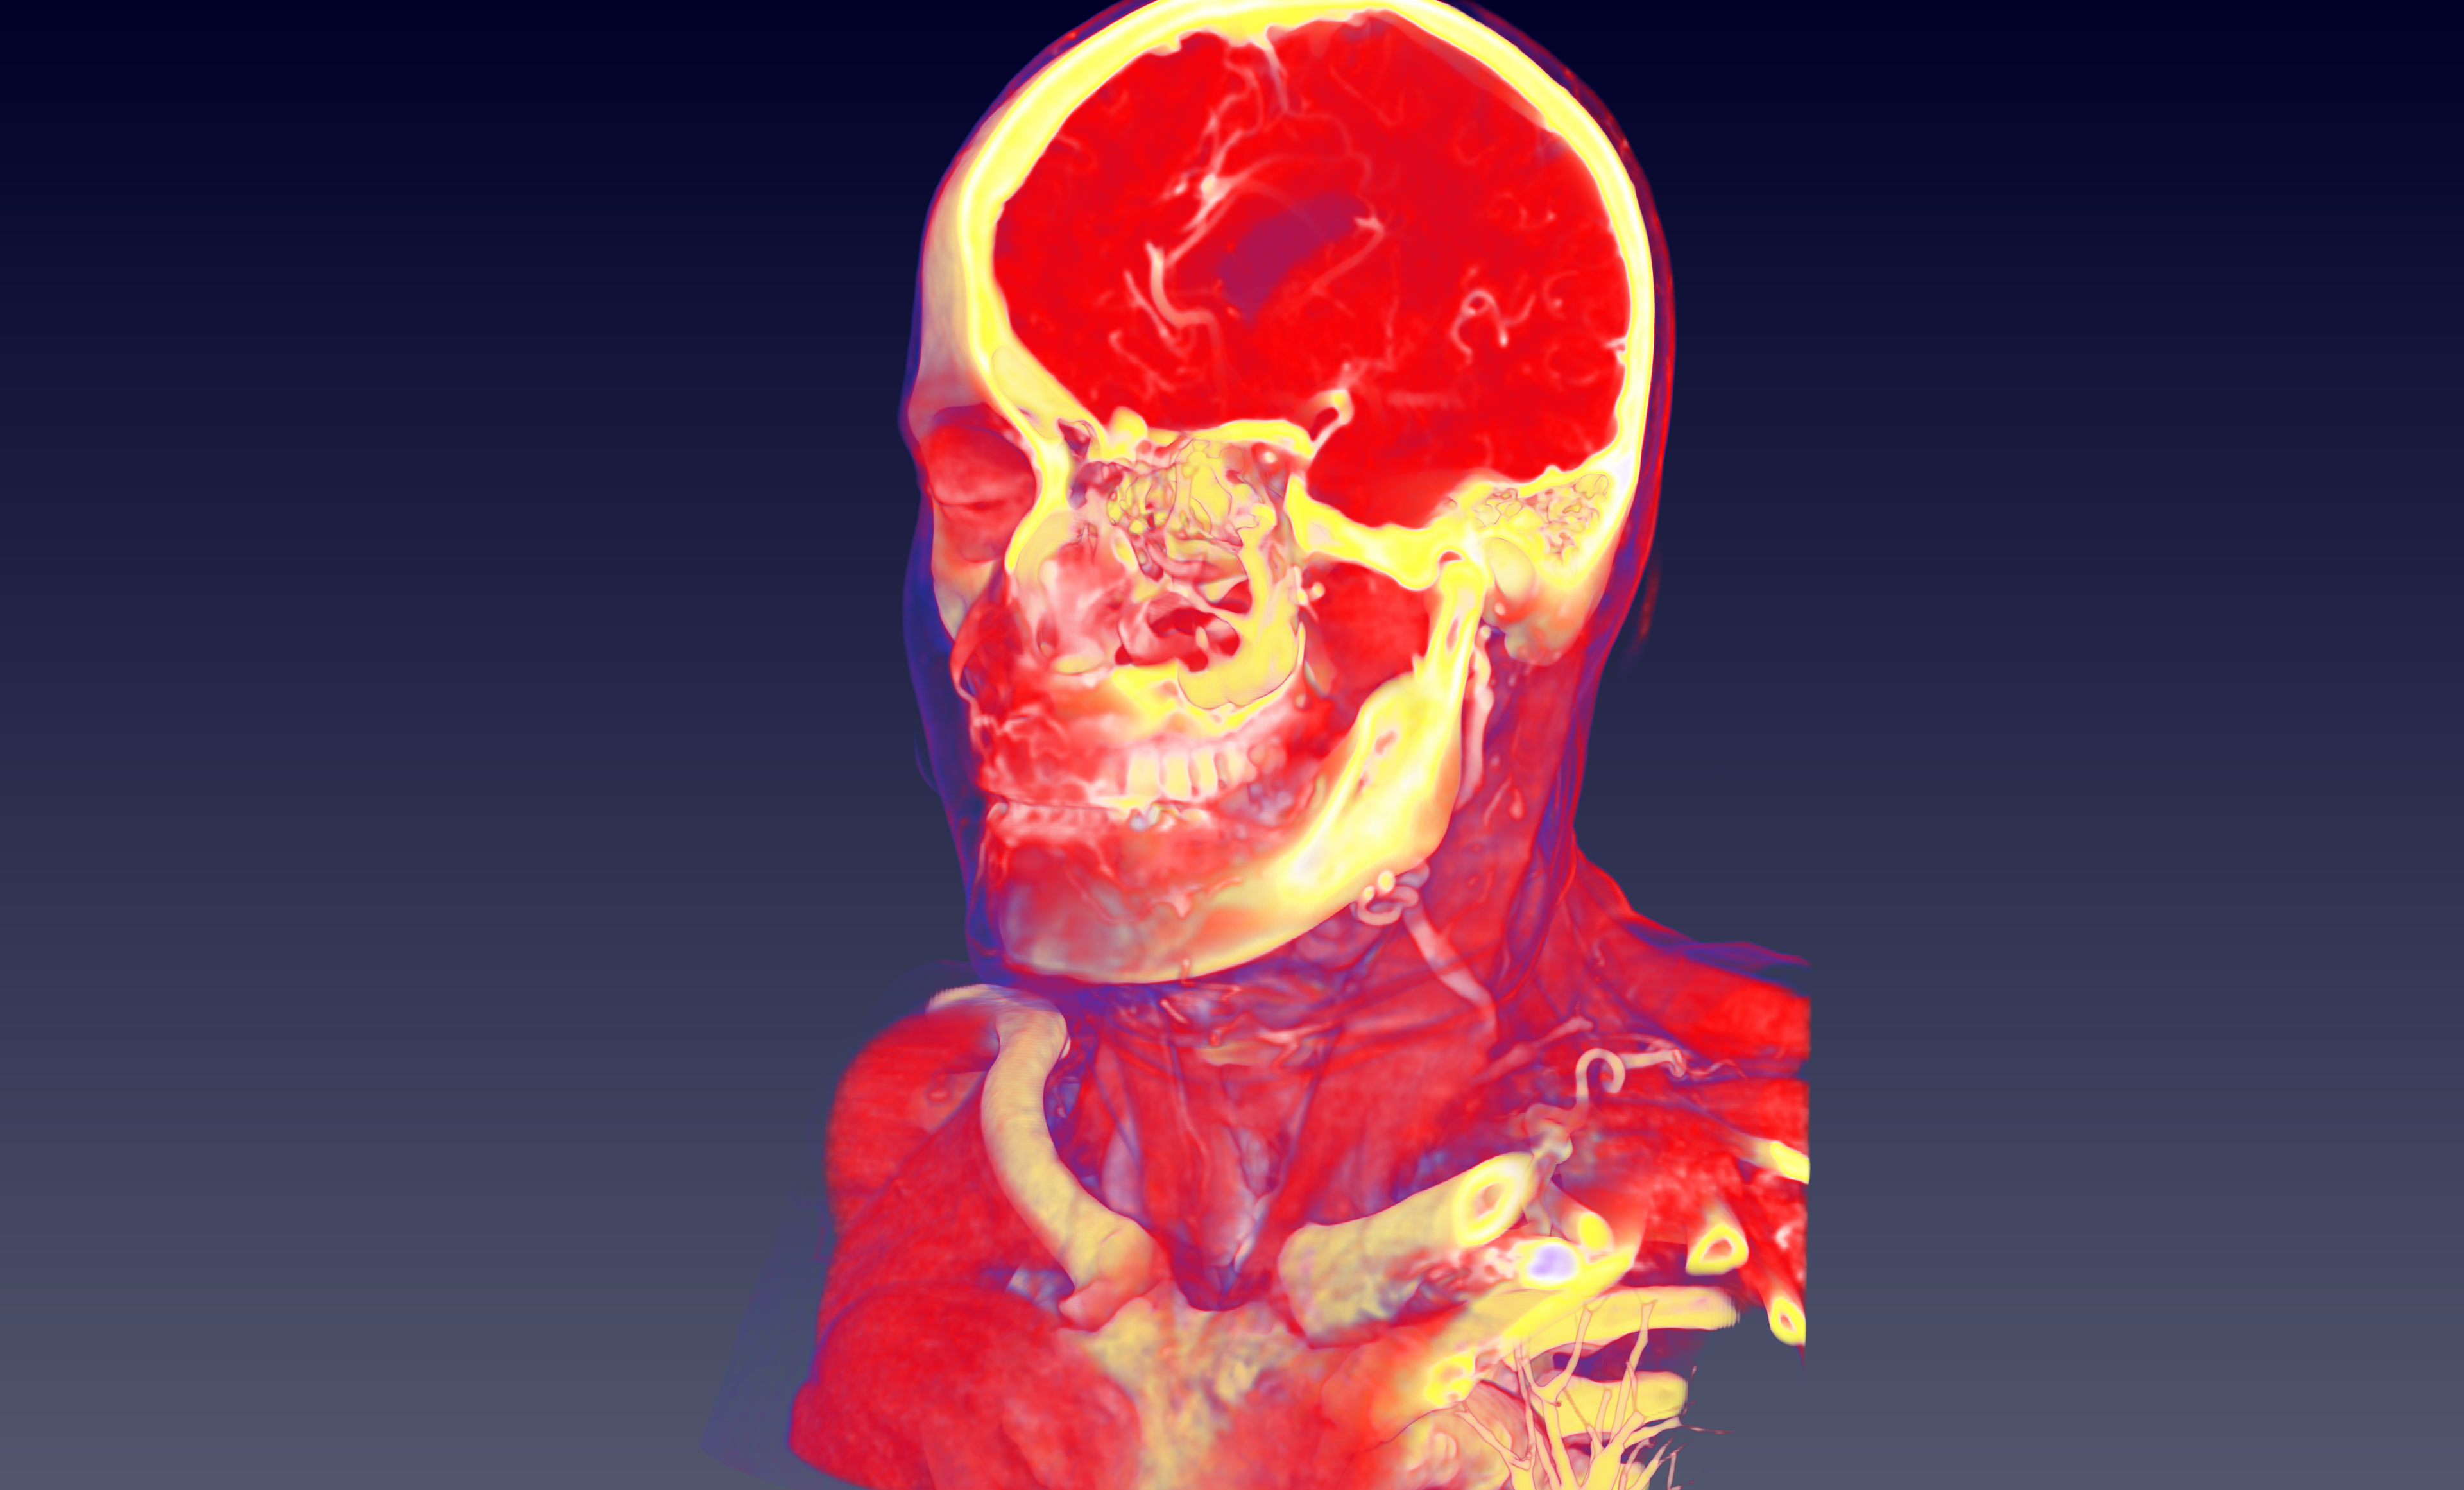
\includegraphics[width=\textwidth]{HeadClippingOblique.png}
    \caption{Clipping using an oblique clipping plane}
    \label{fig:clipoblique}
  \end{subfigure}
  \begin{subfigure}[b]{.5\columnwidth}
    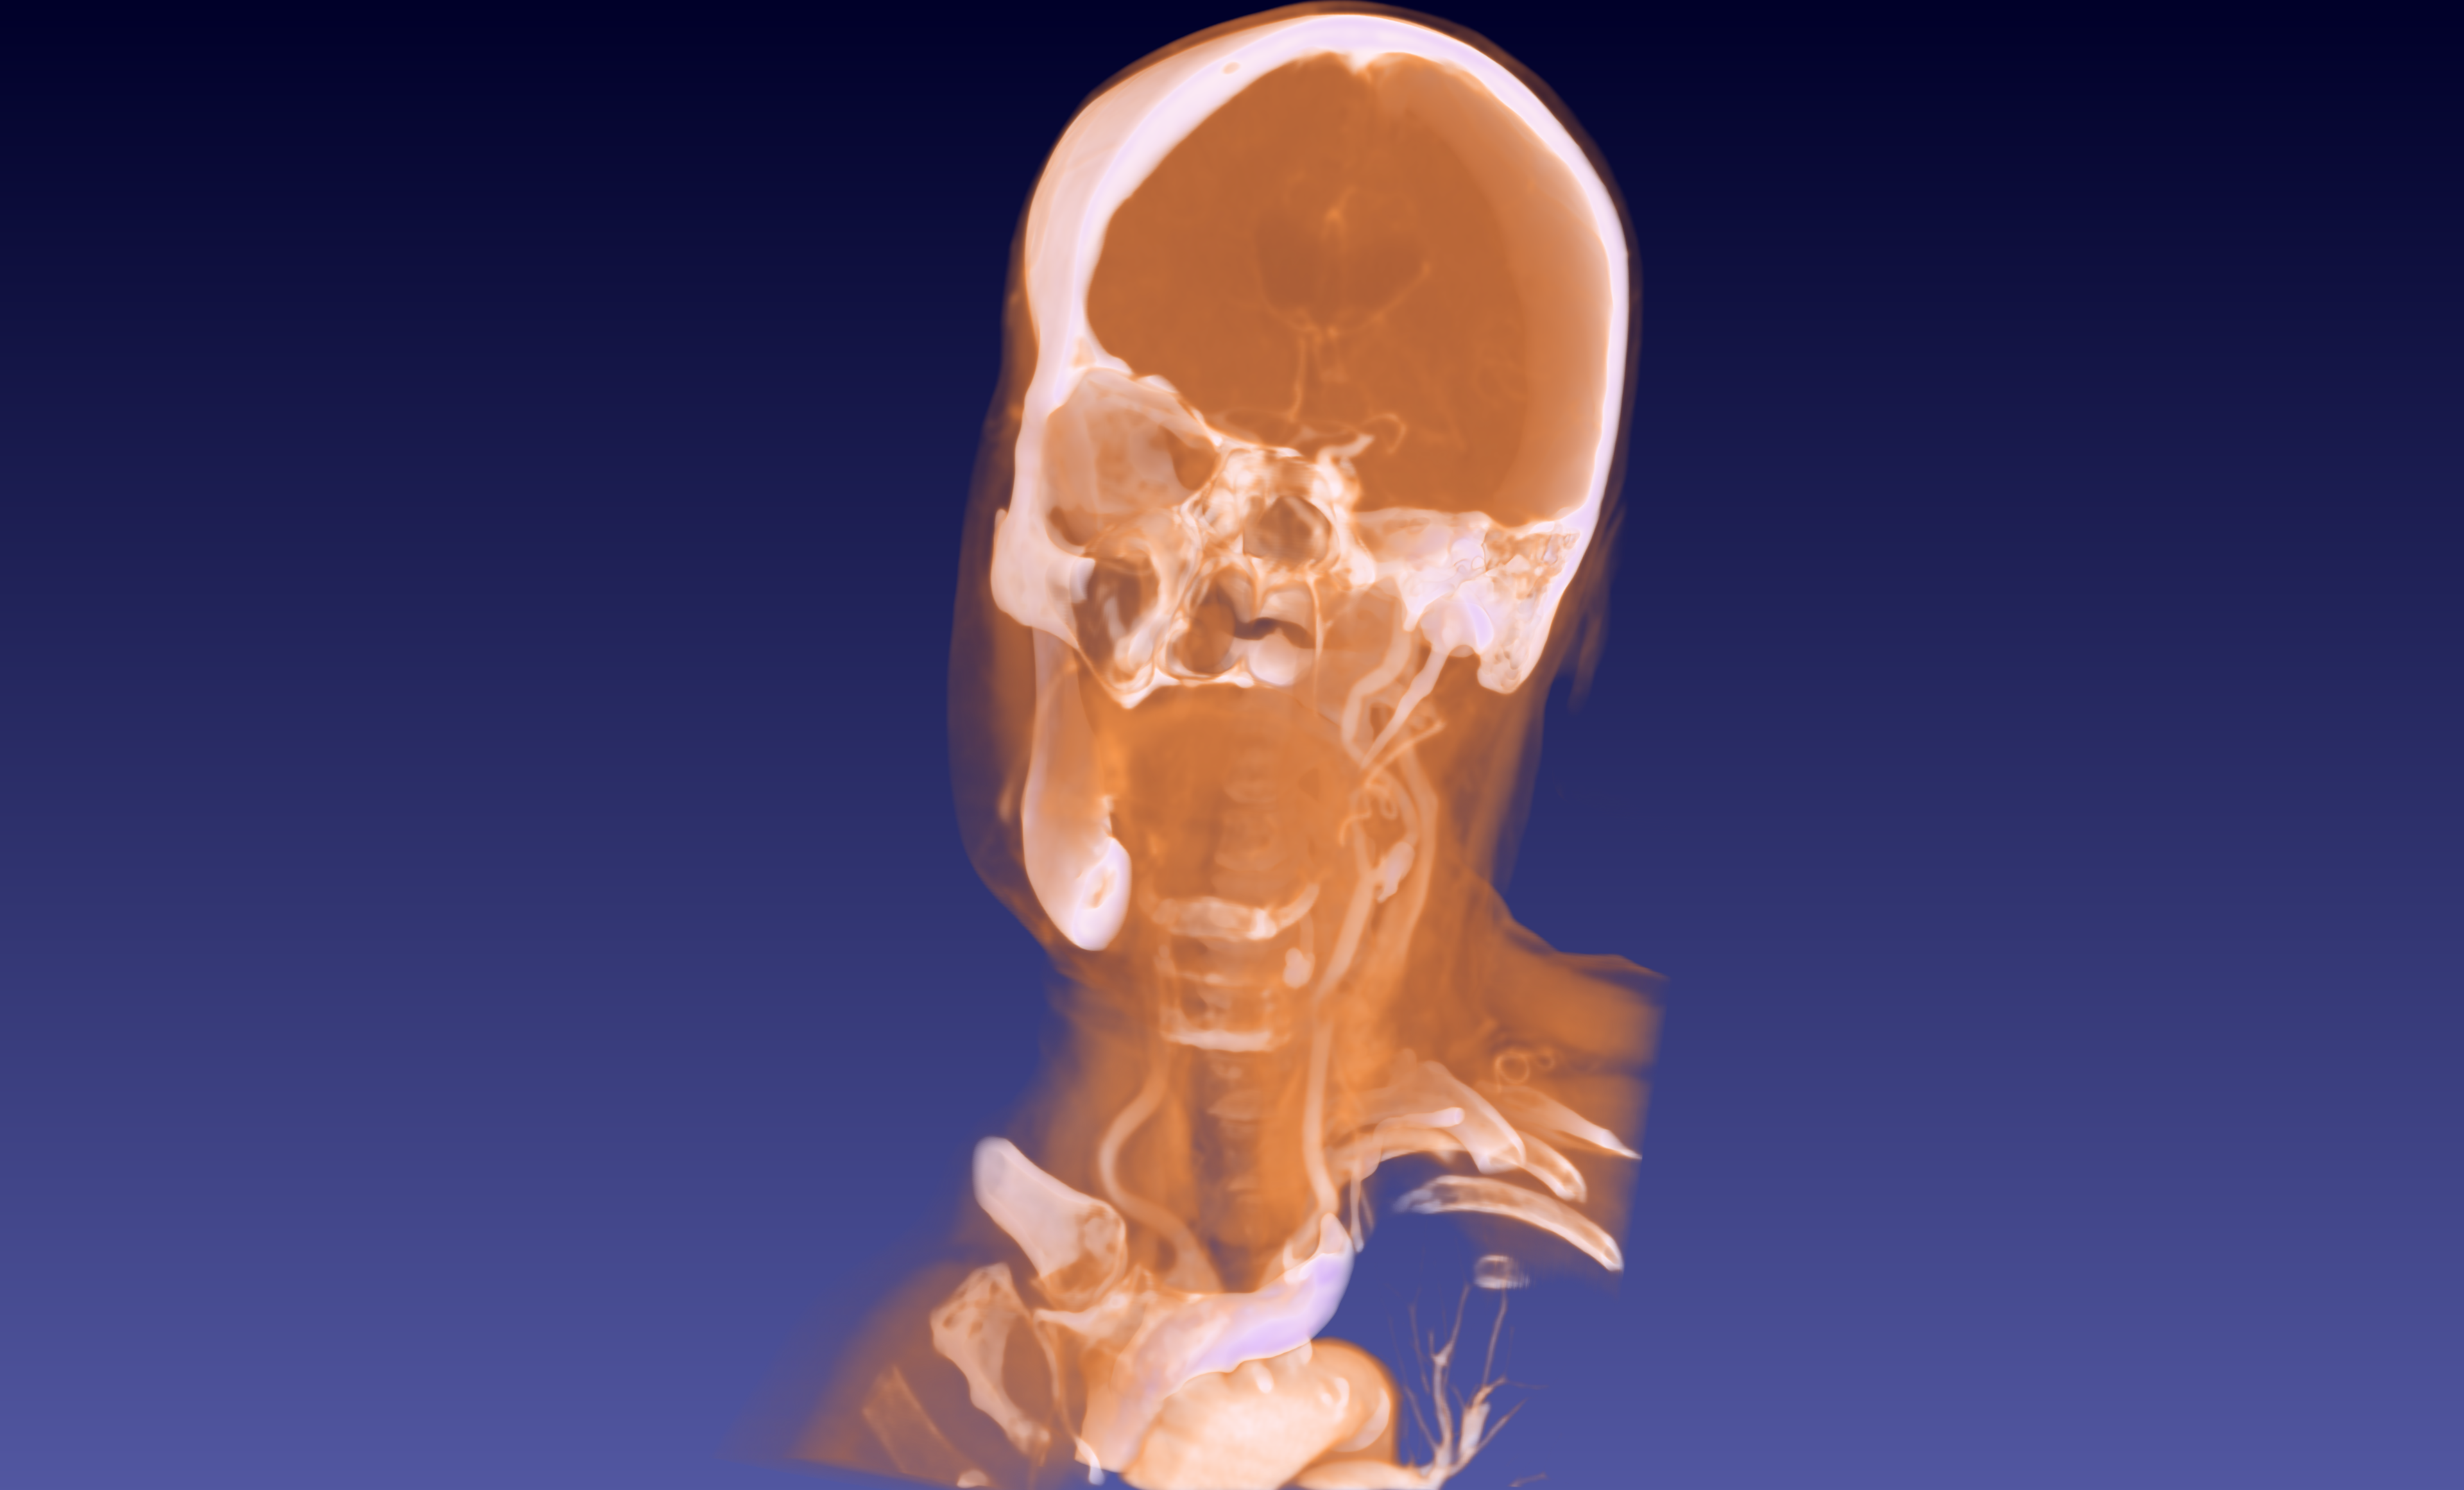
\includegraphics[width=\textwidth]{HeadClippingSlabNoShading.png}
    \caption{Without shading}
    \label{fig:clipnoshading}
  \end{subfigure}%
  \begin{subfigure}[b]{.5\columnwidth}
    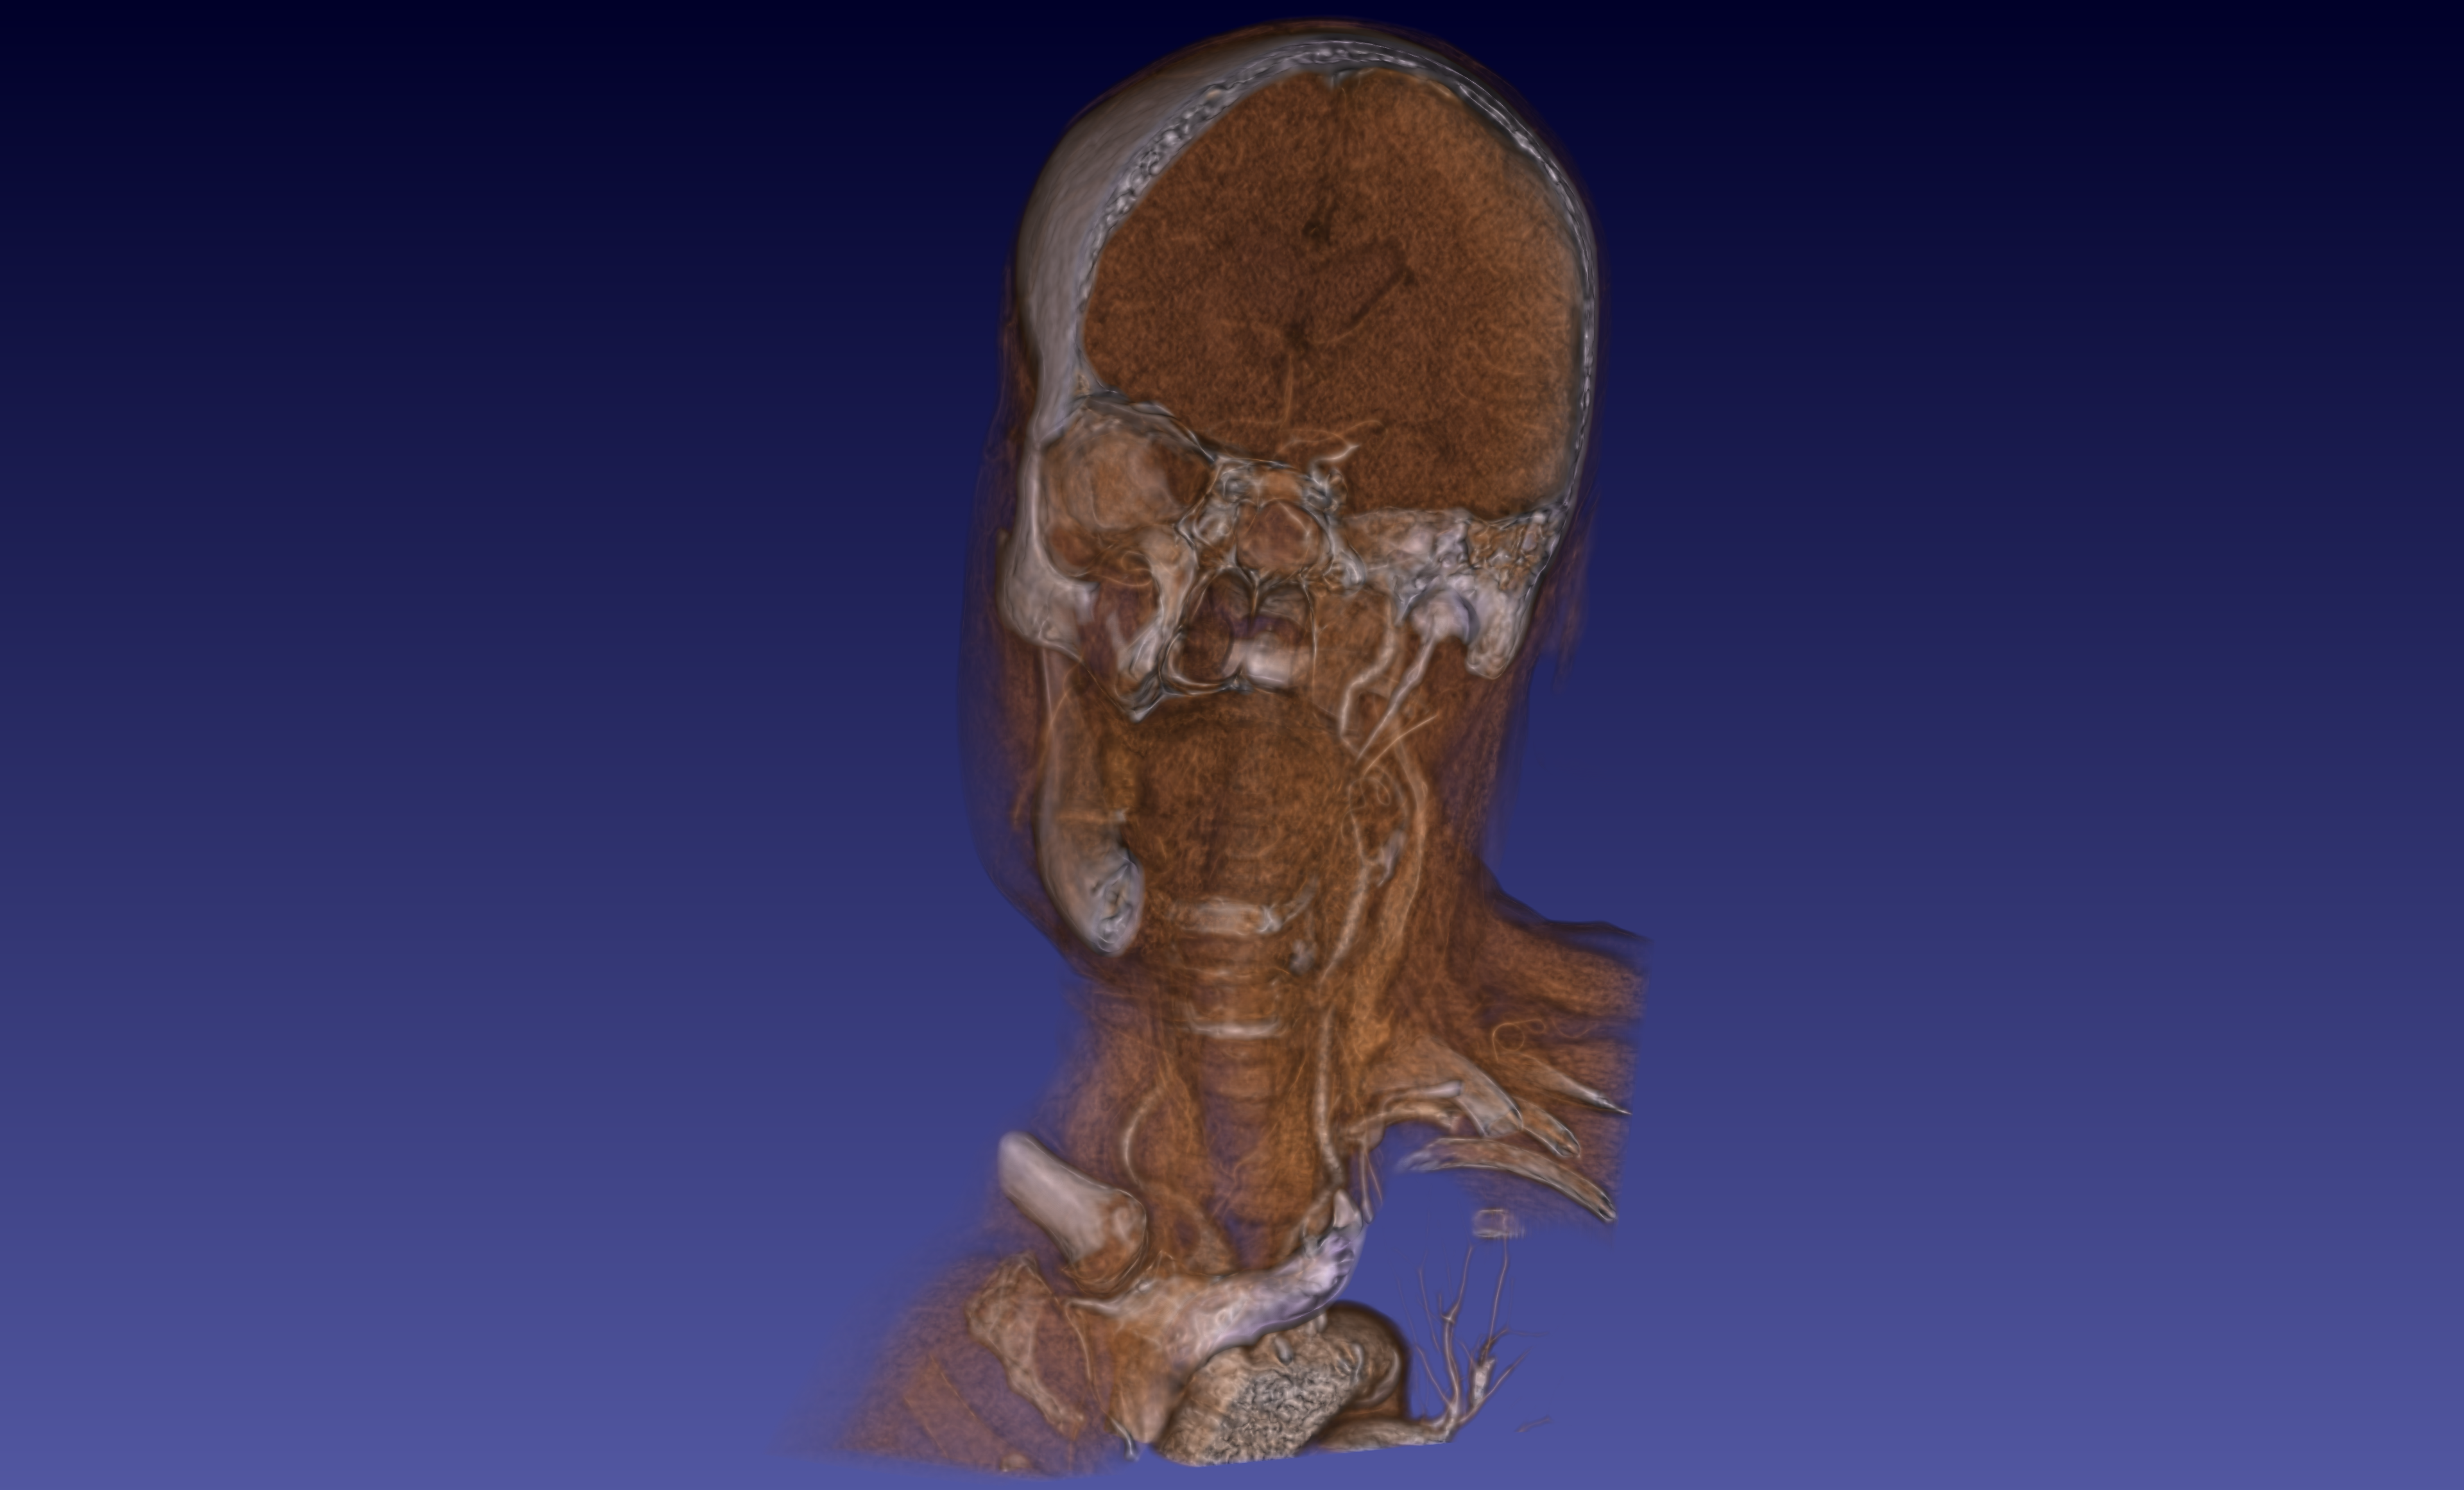
\includegraphics[width=\textwidth]{HeadClippingSlabShading.png}
    \caption{With shading}
    \label{fig:clipshading}
  \end{subfigure}
  \caption{Clipping planes with \texttt{vtkGPUVolumeRayCastMapper}}
  \label{fig:clipping}
\end{figure}

\subsection{Blending Modes}
\label{blending-modes}
The mapper supports composite blending, minimum intensity projection, maximum
intensity projection, additive intensity and average intensity blending. Each of
these blending modes are useful for a particular use-case in medical computing.
The most common one which is also the default is the composite blending mode.
See ~\Autoref{fig:blendingmodes} for an example of the different blend modes
on the same data.

\begin{figure}[htb]
  \centering%
  \begin{subfigure}{.5\columnwidth}
    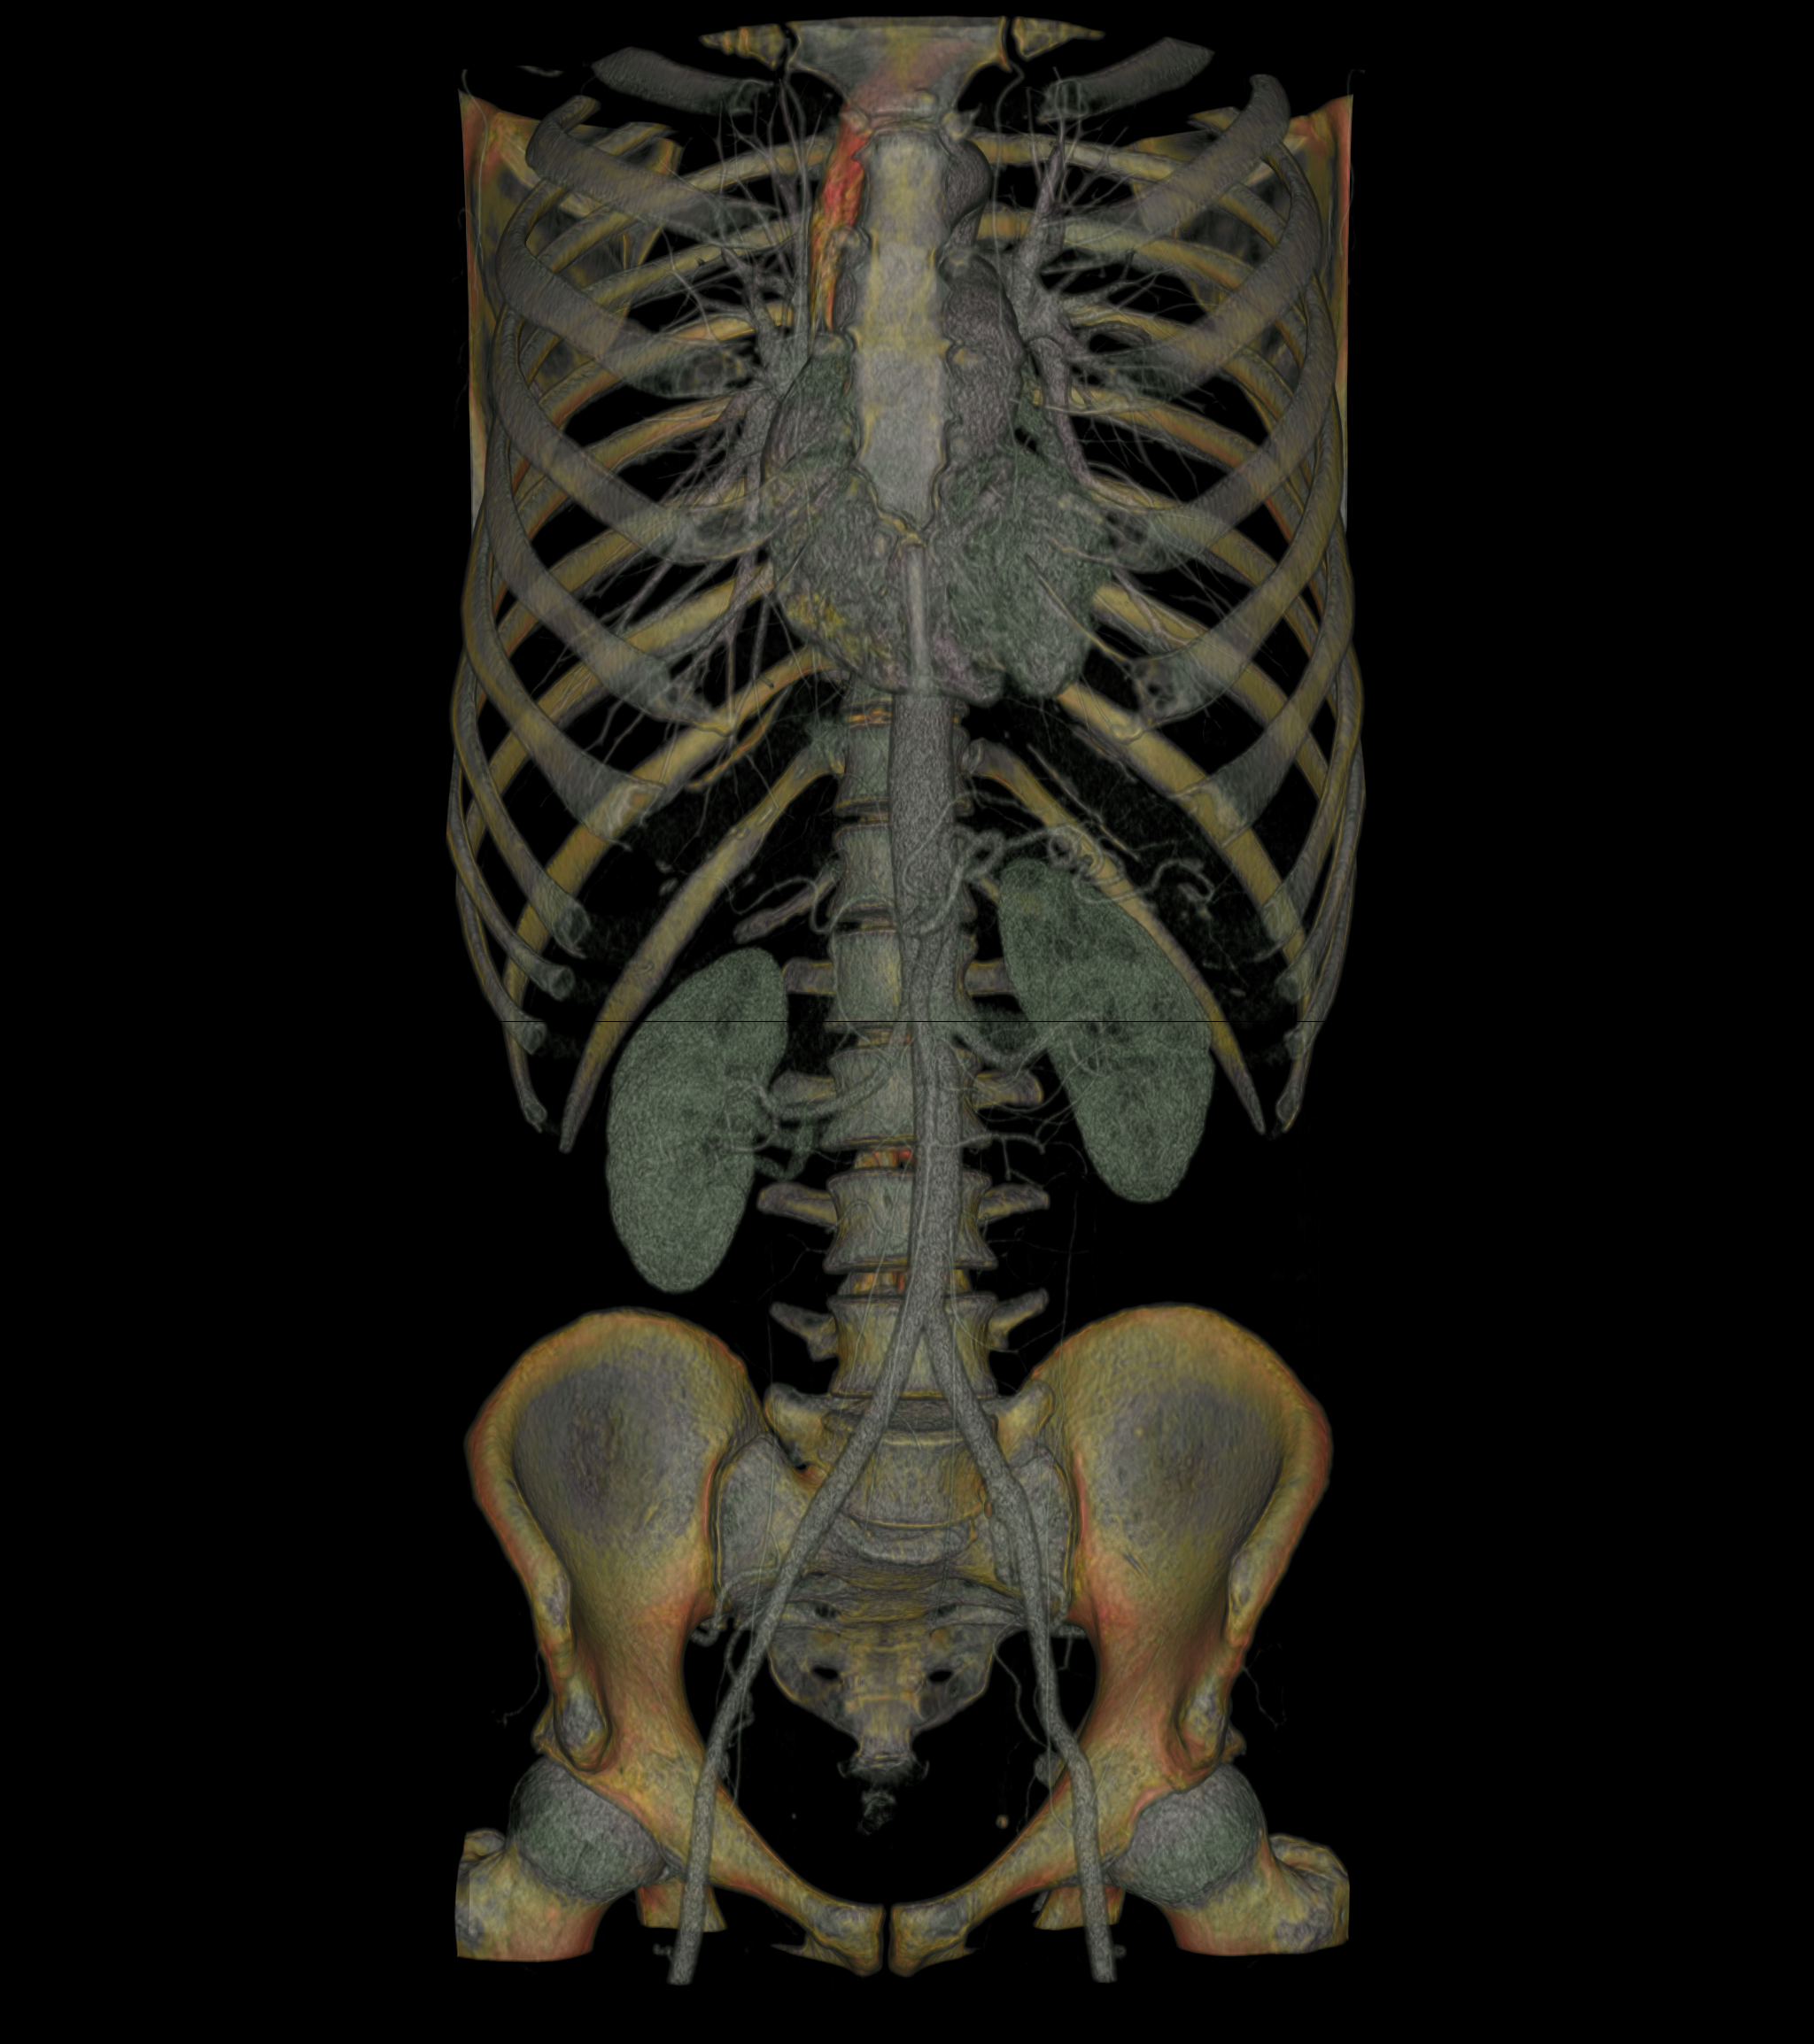
\includegraphics[width=\columnwidth]{TorsoBlendingComposite.png}
    \caption{Composite}
    \label{fig:blendcomposite}
  \end{subfigure}%
  \begin{subfigure}{.5\columnwidth}
    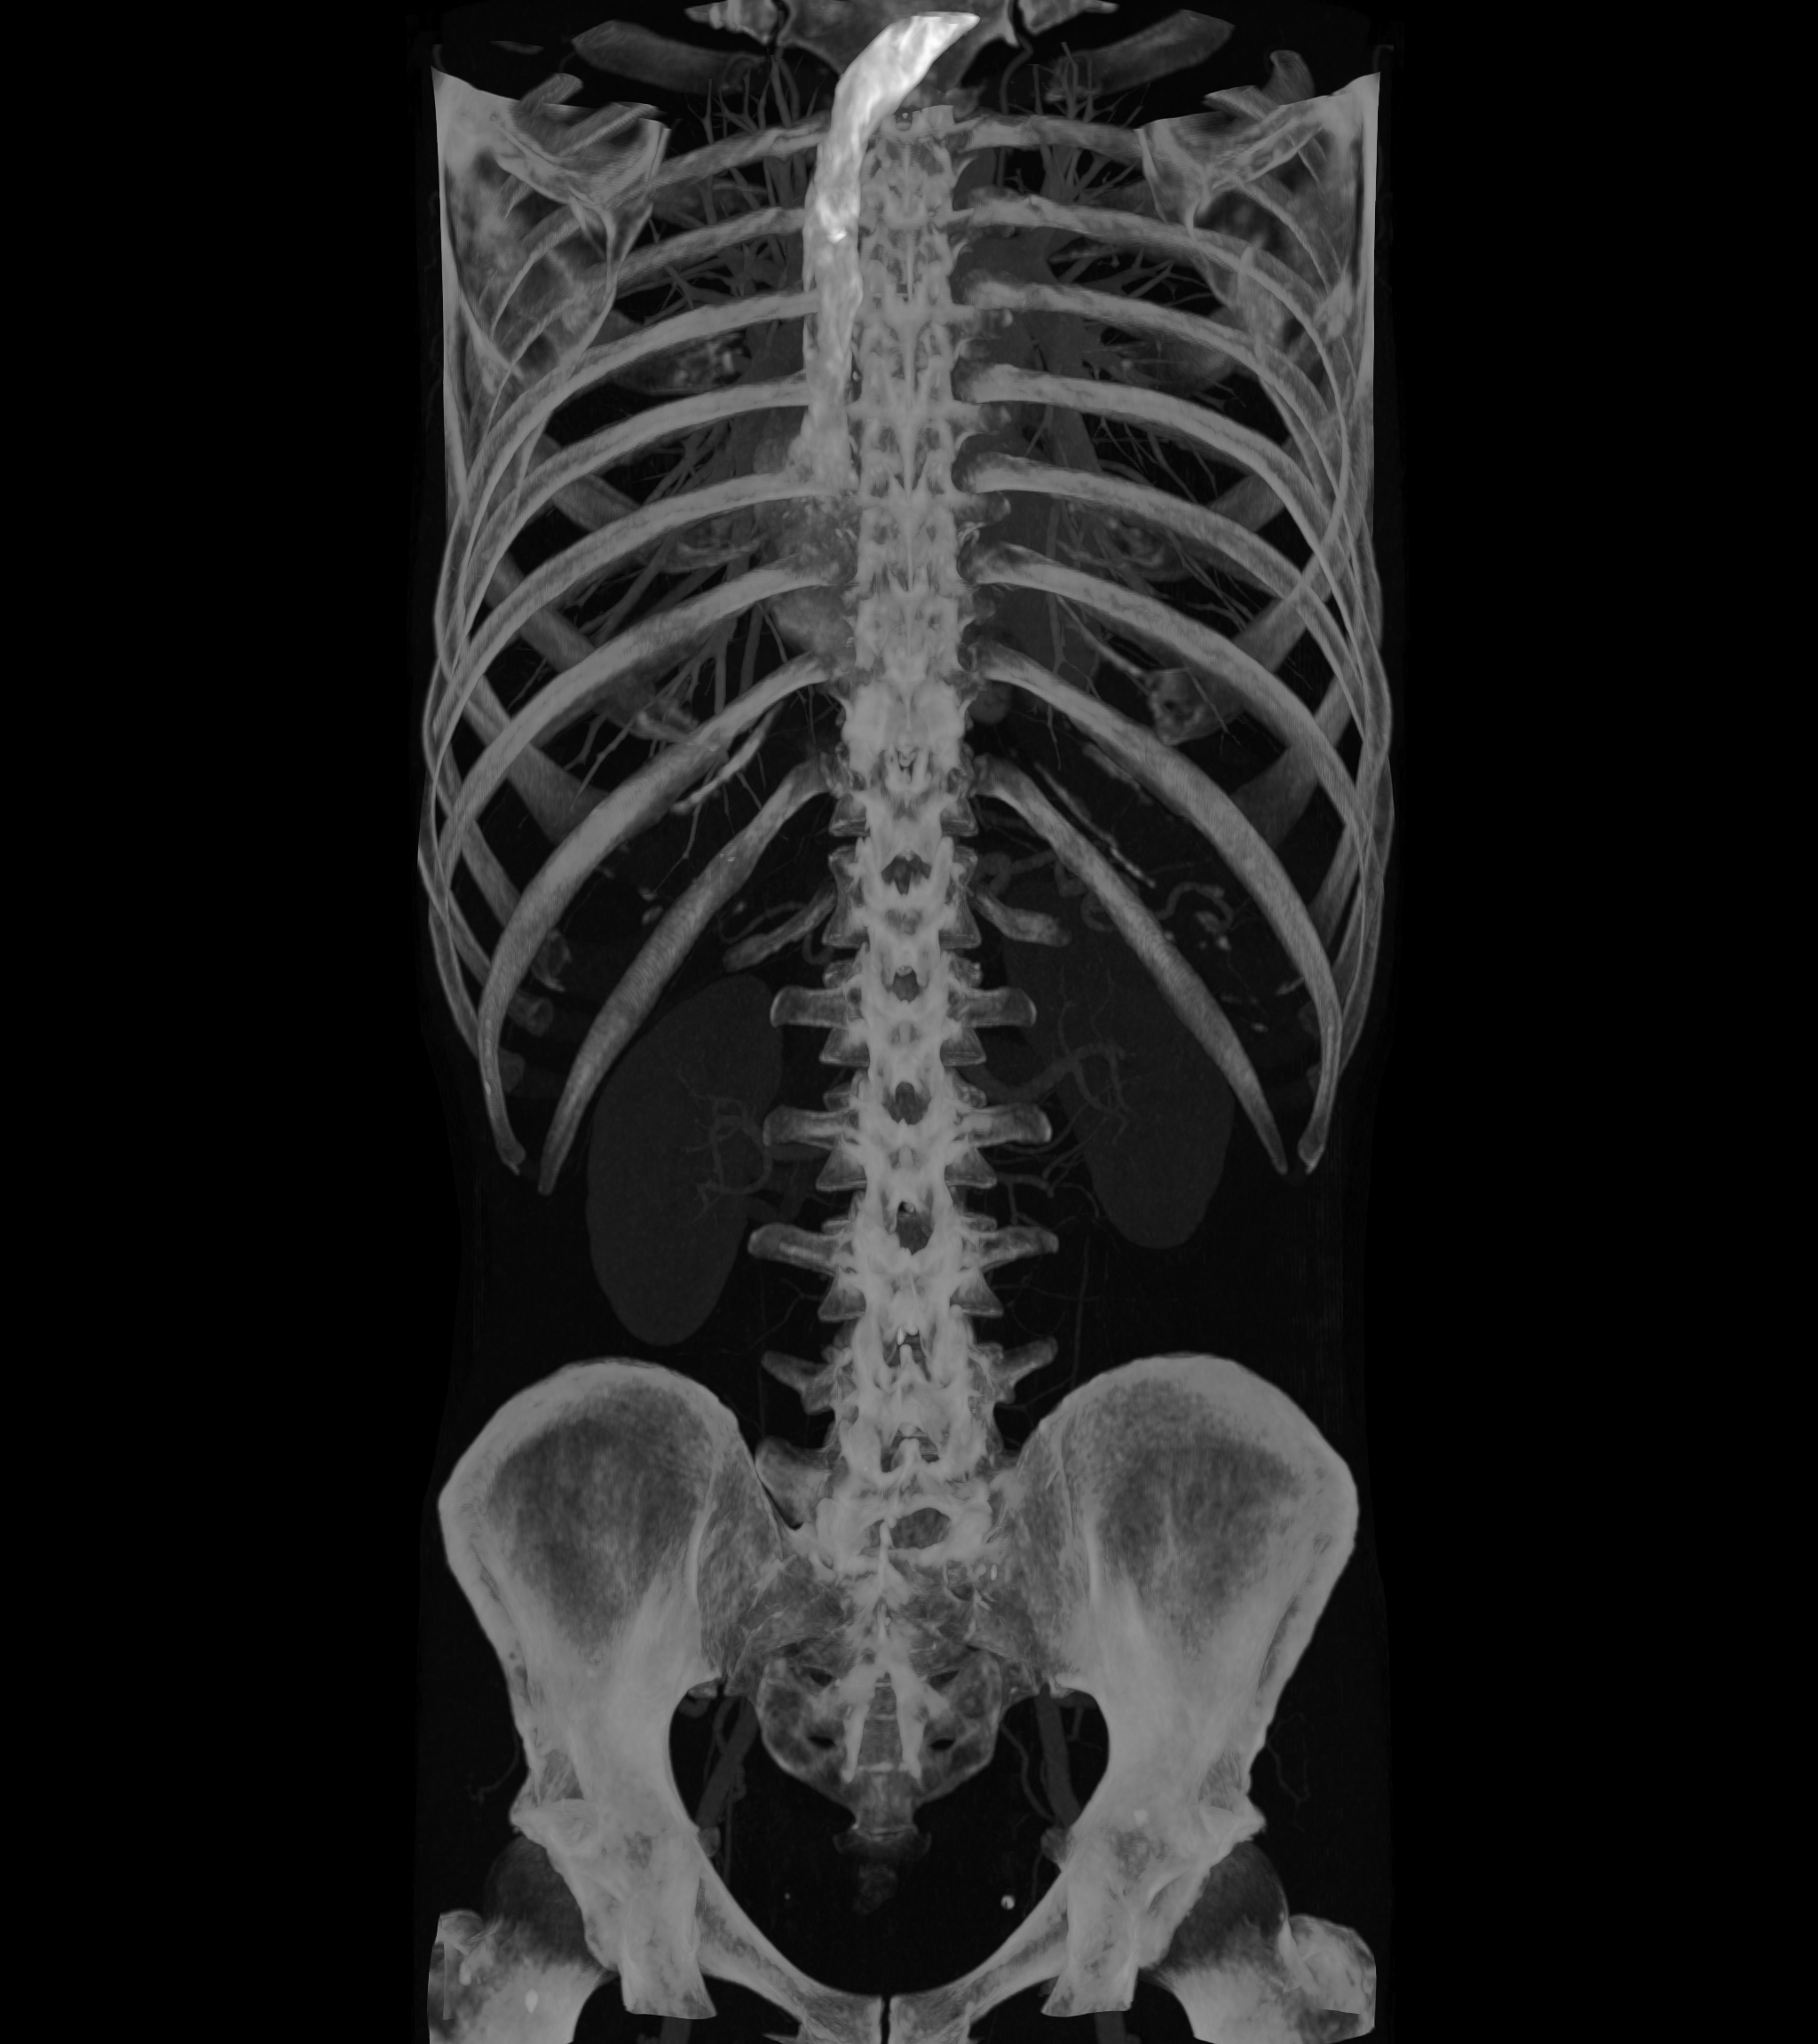
\includegraphics[width=\columnwidth]{TorsoBlendingMIP.png}
    \caption{Maximum Intensity}
    \label{fig:blendmax}
  \end{subfigure}
  \begin{subfigure}{.5\columnwidth}
    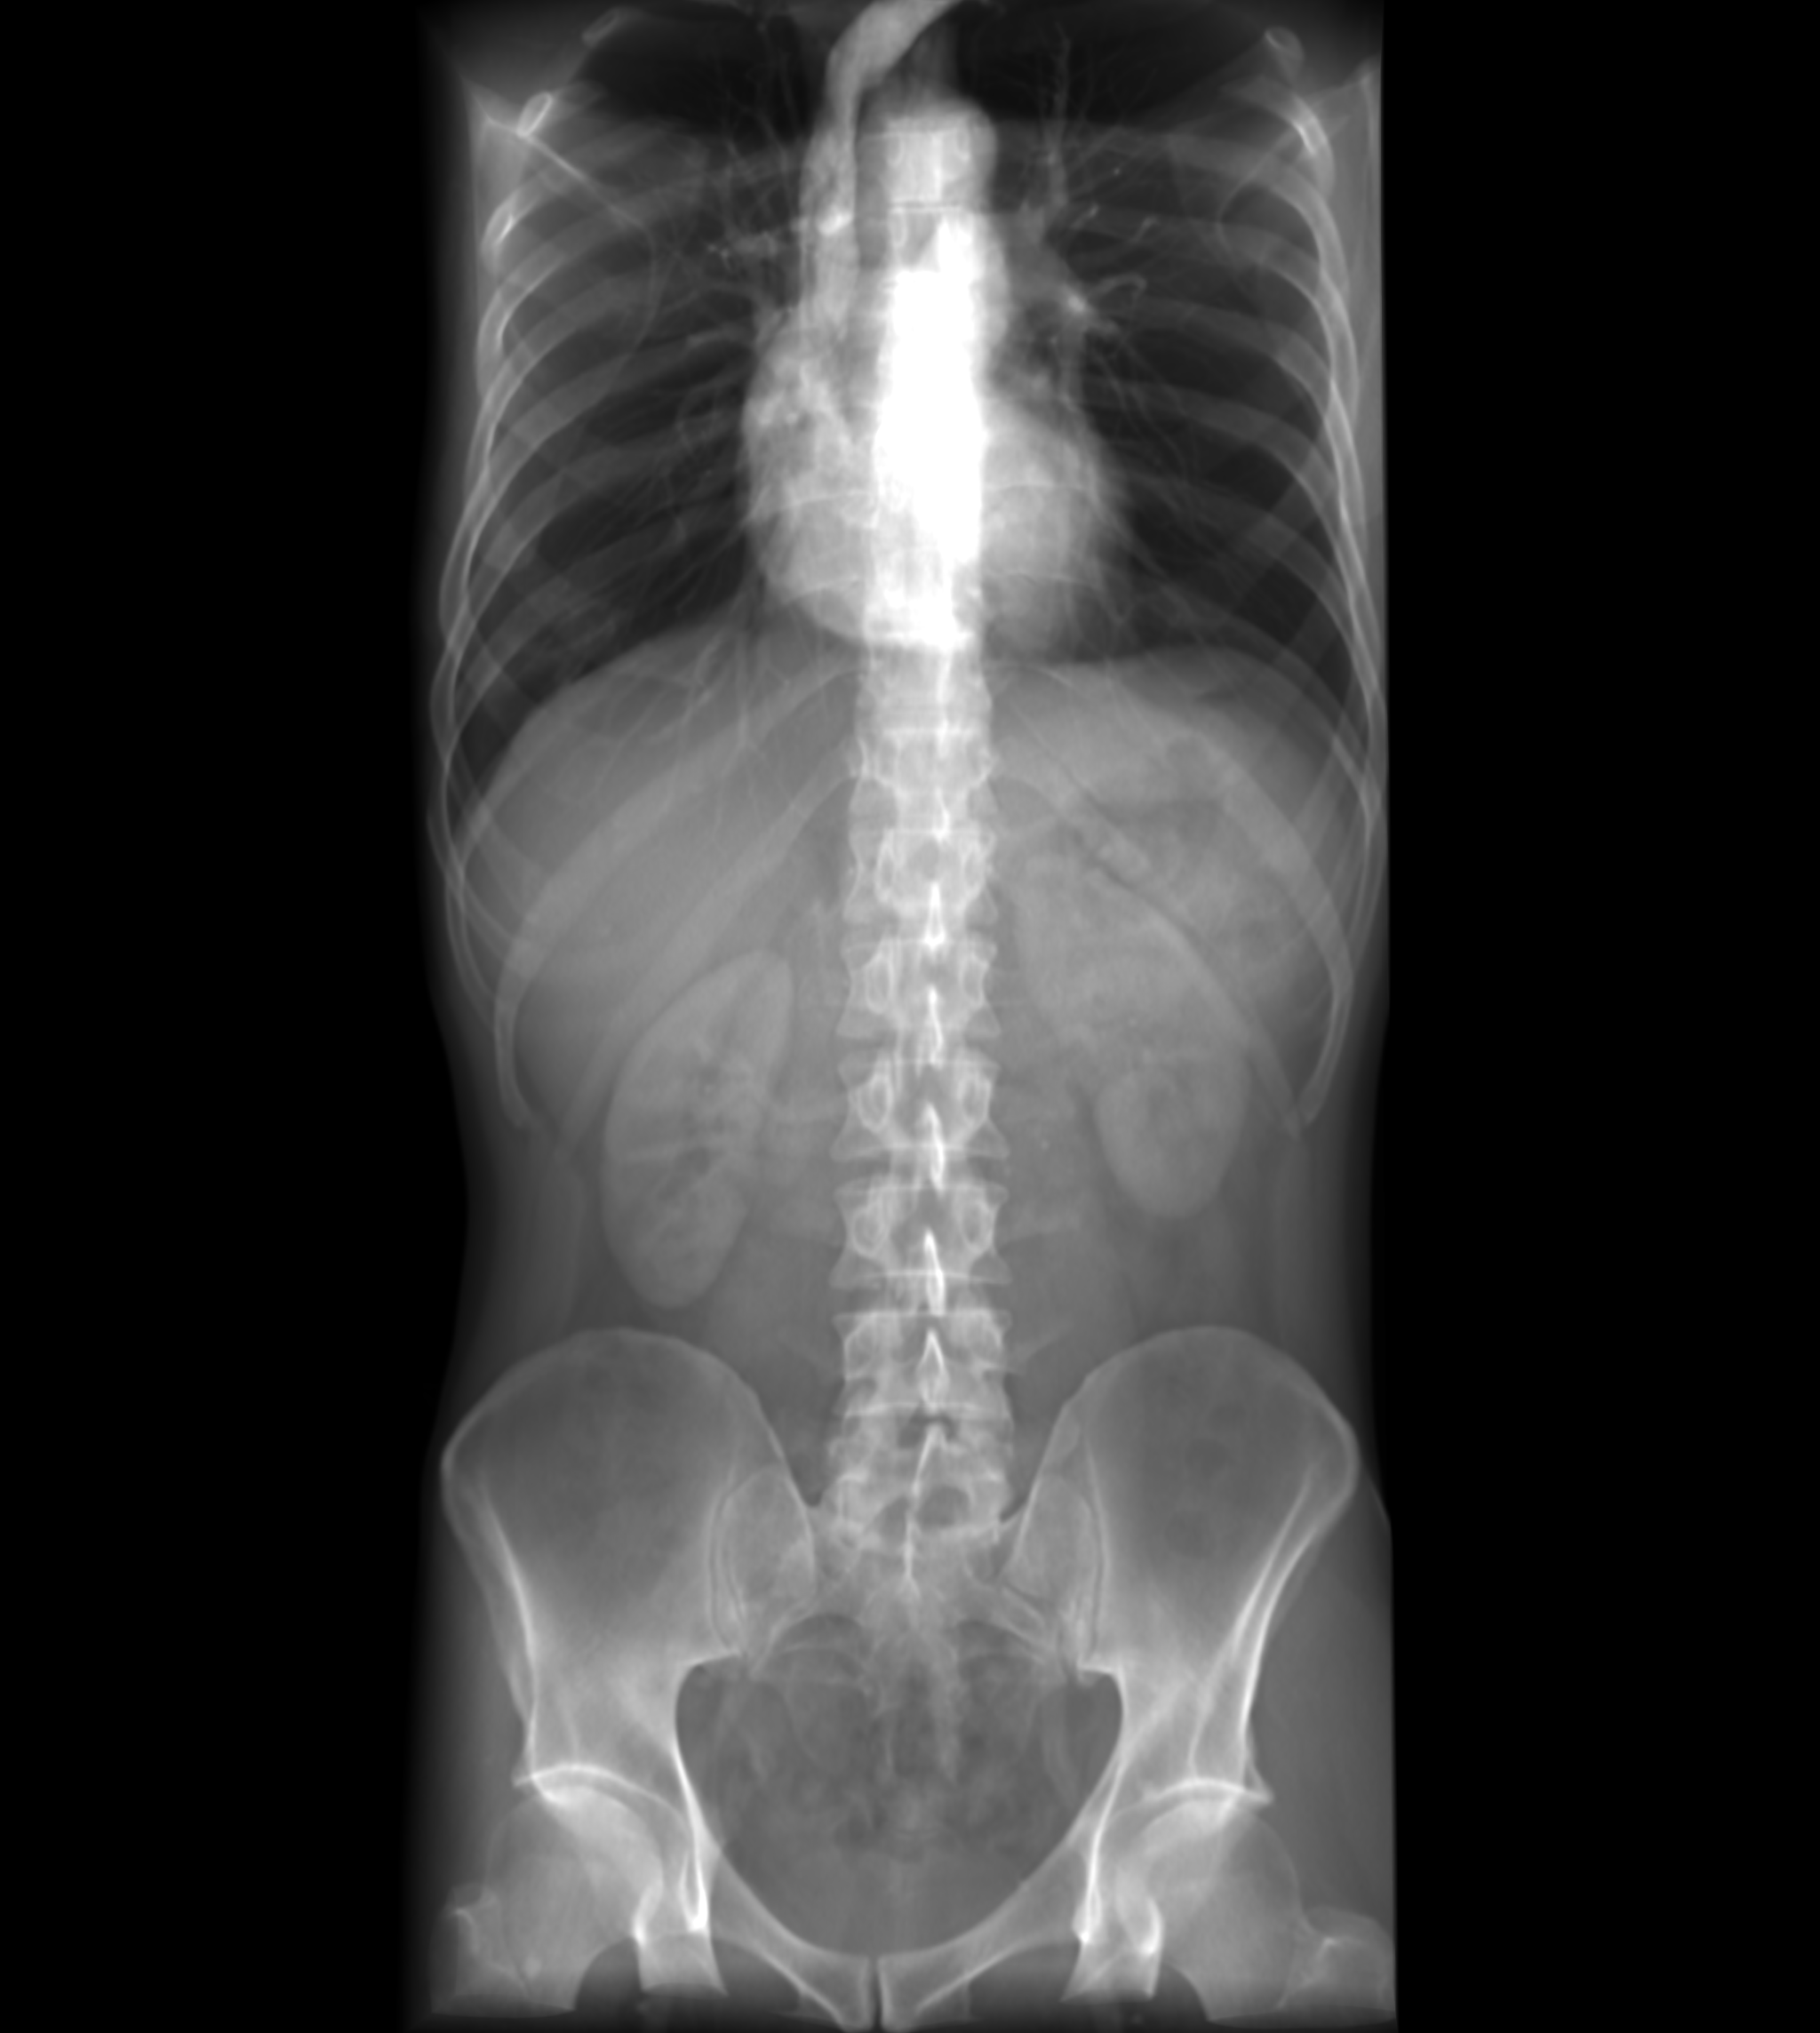
\includegraphics[width=\columnwidth]{TorsoBlendingAdditive.png}
    \caption{Additive}
    \label{fig:blendadditive}
  \end{subfigure}%
  \begin{subfigure}{.5\columnwidth}
    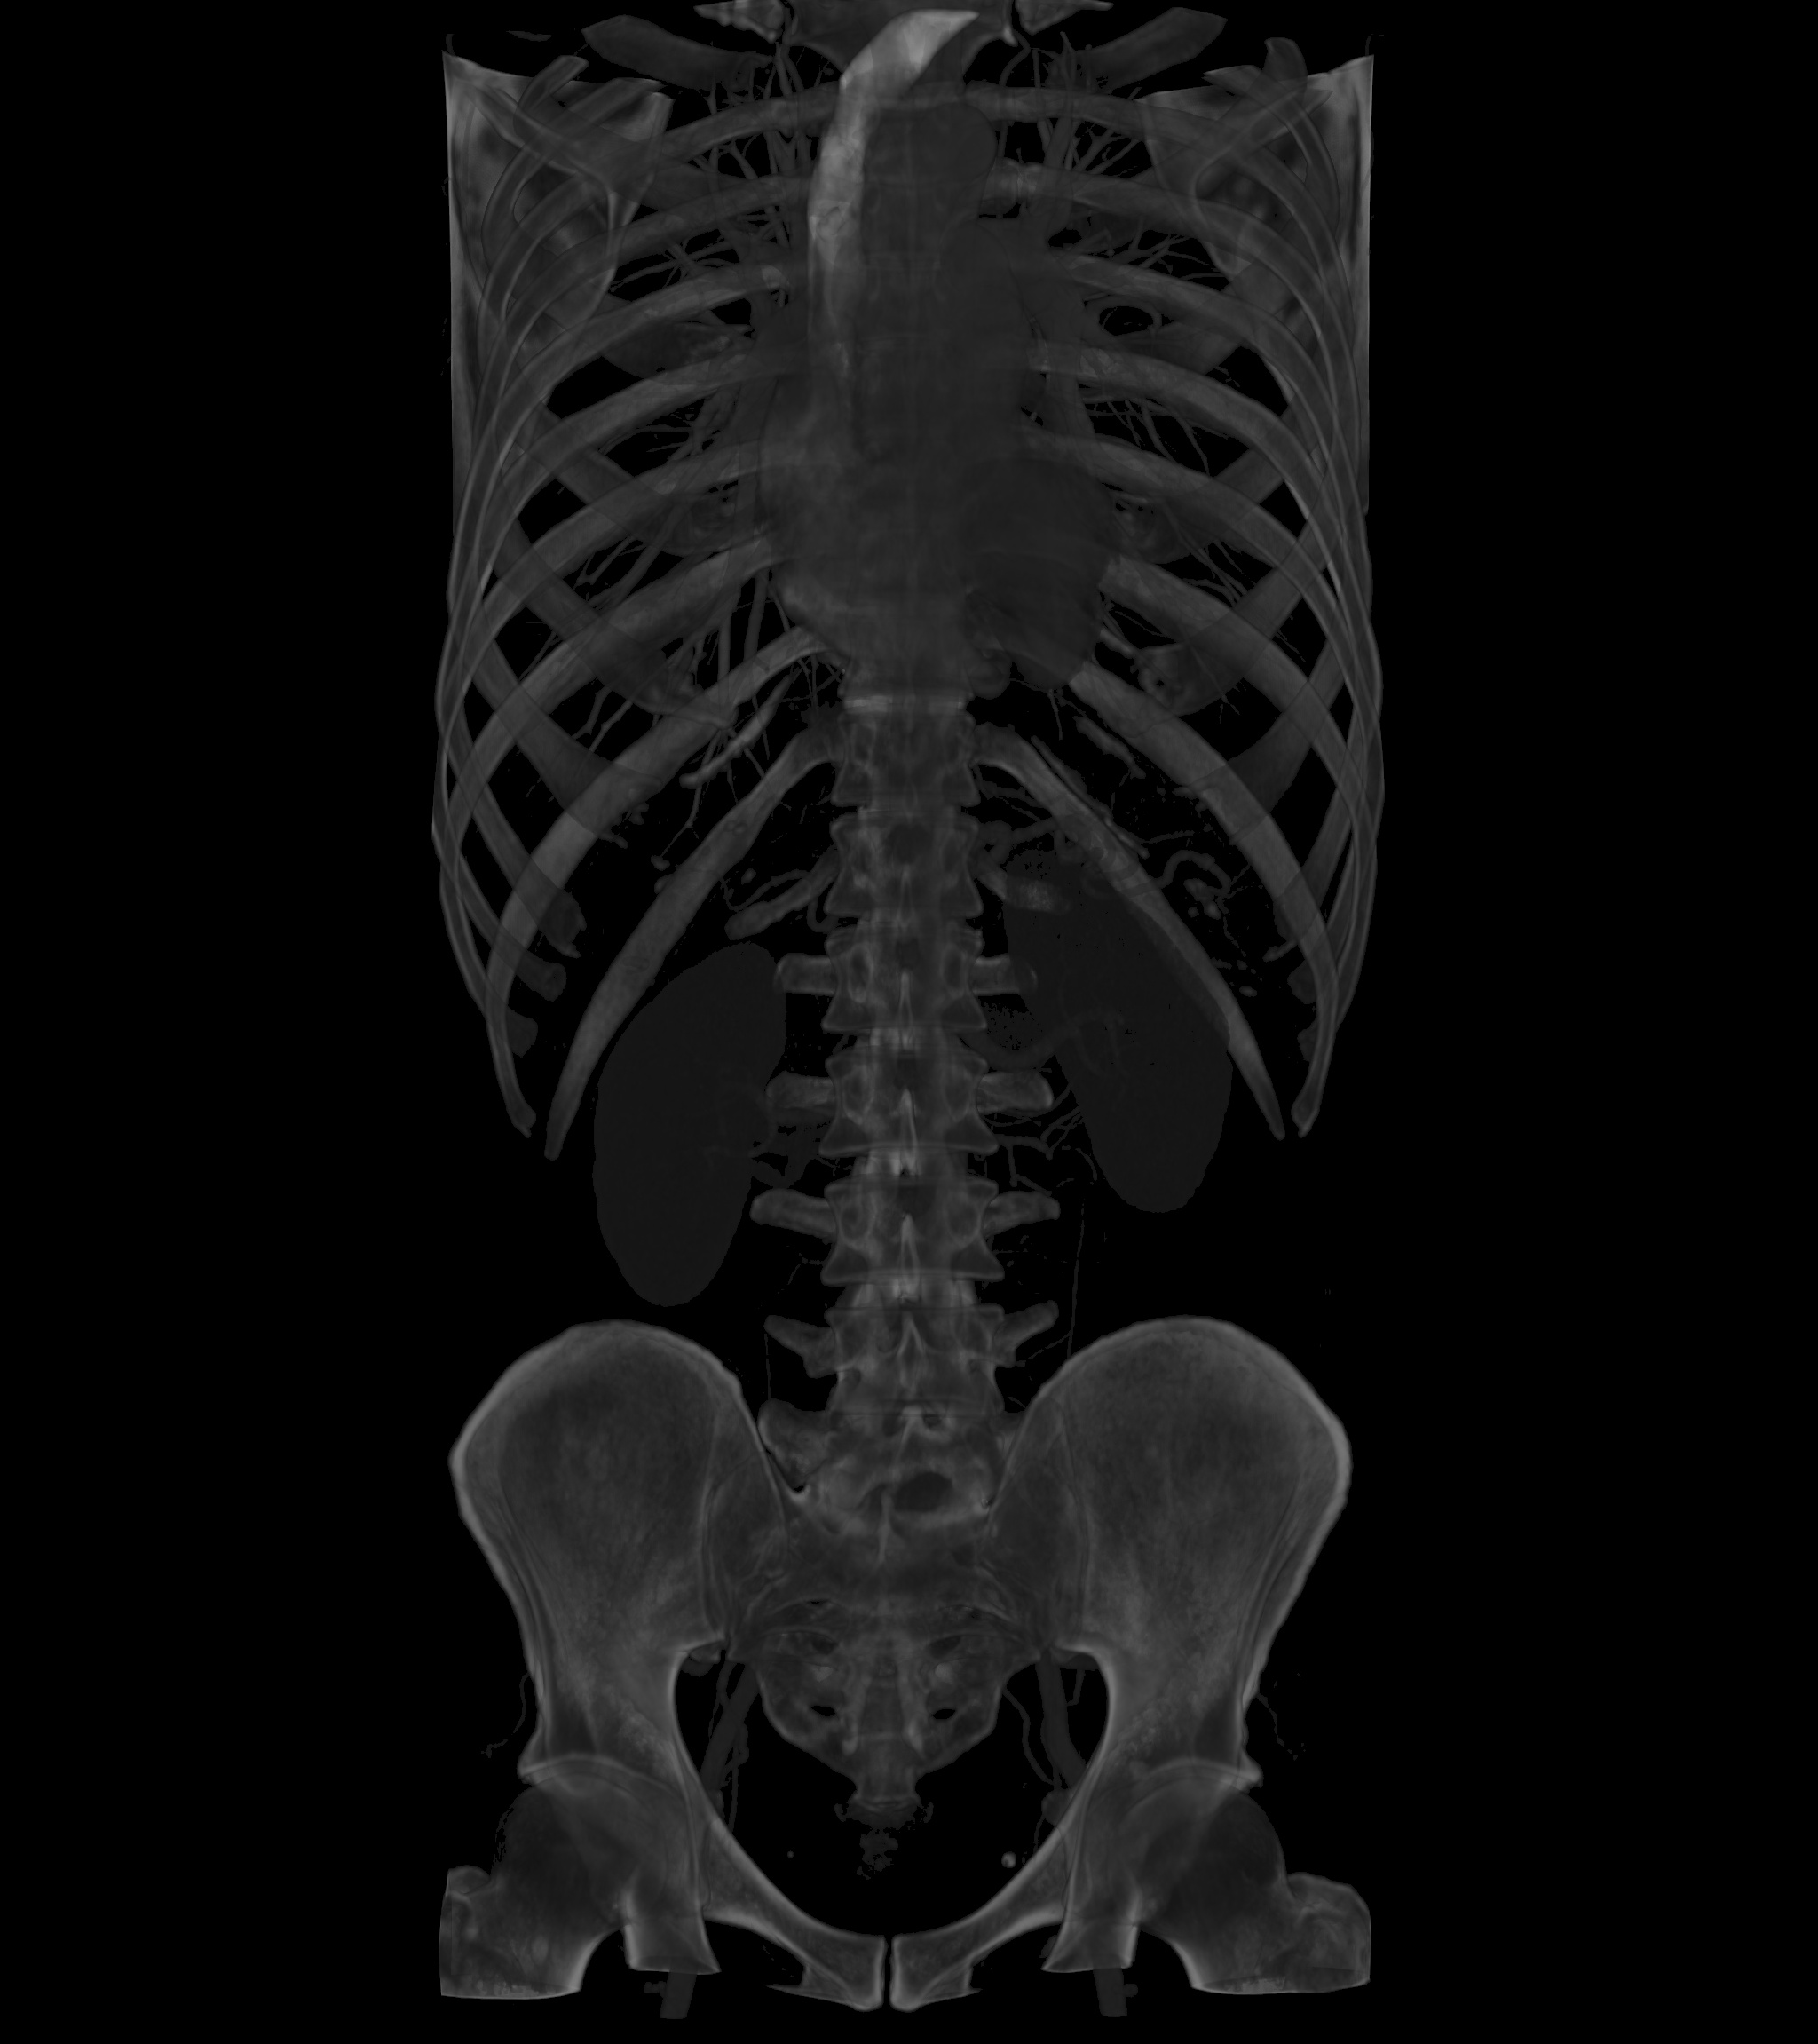
\includegraphics[width=\columnwidth]{TorsoBlendingAverage.png}
    \caption{Average Intensity}
    \label{fig:blendaverage}
  \end{subfigure}%
  \caption{Blend modes supported by \texttt{vtkGPUVolumeRayCastMapper}}
  \label{fig:blendingmodes}
\end{figure}

\subsection{Masking}
\label{masking}
Both binary and label masks are supported. With binary masks, the value in the
masking volume indicates visibility of the voxel in the data volume. When a
label map is in use, the value in the label map is used to select different
rendering parameters for that sample.  See Figure 5 for an example of label data
masks.

\subsection{Opacity Modulated by Gradient Magnitude}
\label{opacity-modulated-by-gradient-magnitude}
While the \texttt{vtkGPUVolumeRayCastMapper} supports direct accumulation of
color and opacity values along the ray, it also allows for modulating the
opacity accumulation calculation based on relative values of each voxel in the
dataset. Prior efforts~\citep{marchesin_per-pixel_2010} have demonstrated the
usefulness of such a technique for feature enhancement in the rendered image. A
transfer function mapping the magnitude of the gradient to an opacity modulation
value can be used to essentially perform edge detection (de-emphasize homogenous
regions) during rendering. See ~\Autoref{fig:gradient} for an example of
rendering with and without the use of a gradient opacity transfer function.

\begin{figure}[htb]
  \centering
   \begin{subfigure}[b]{0.5\columnwidth}
     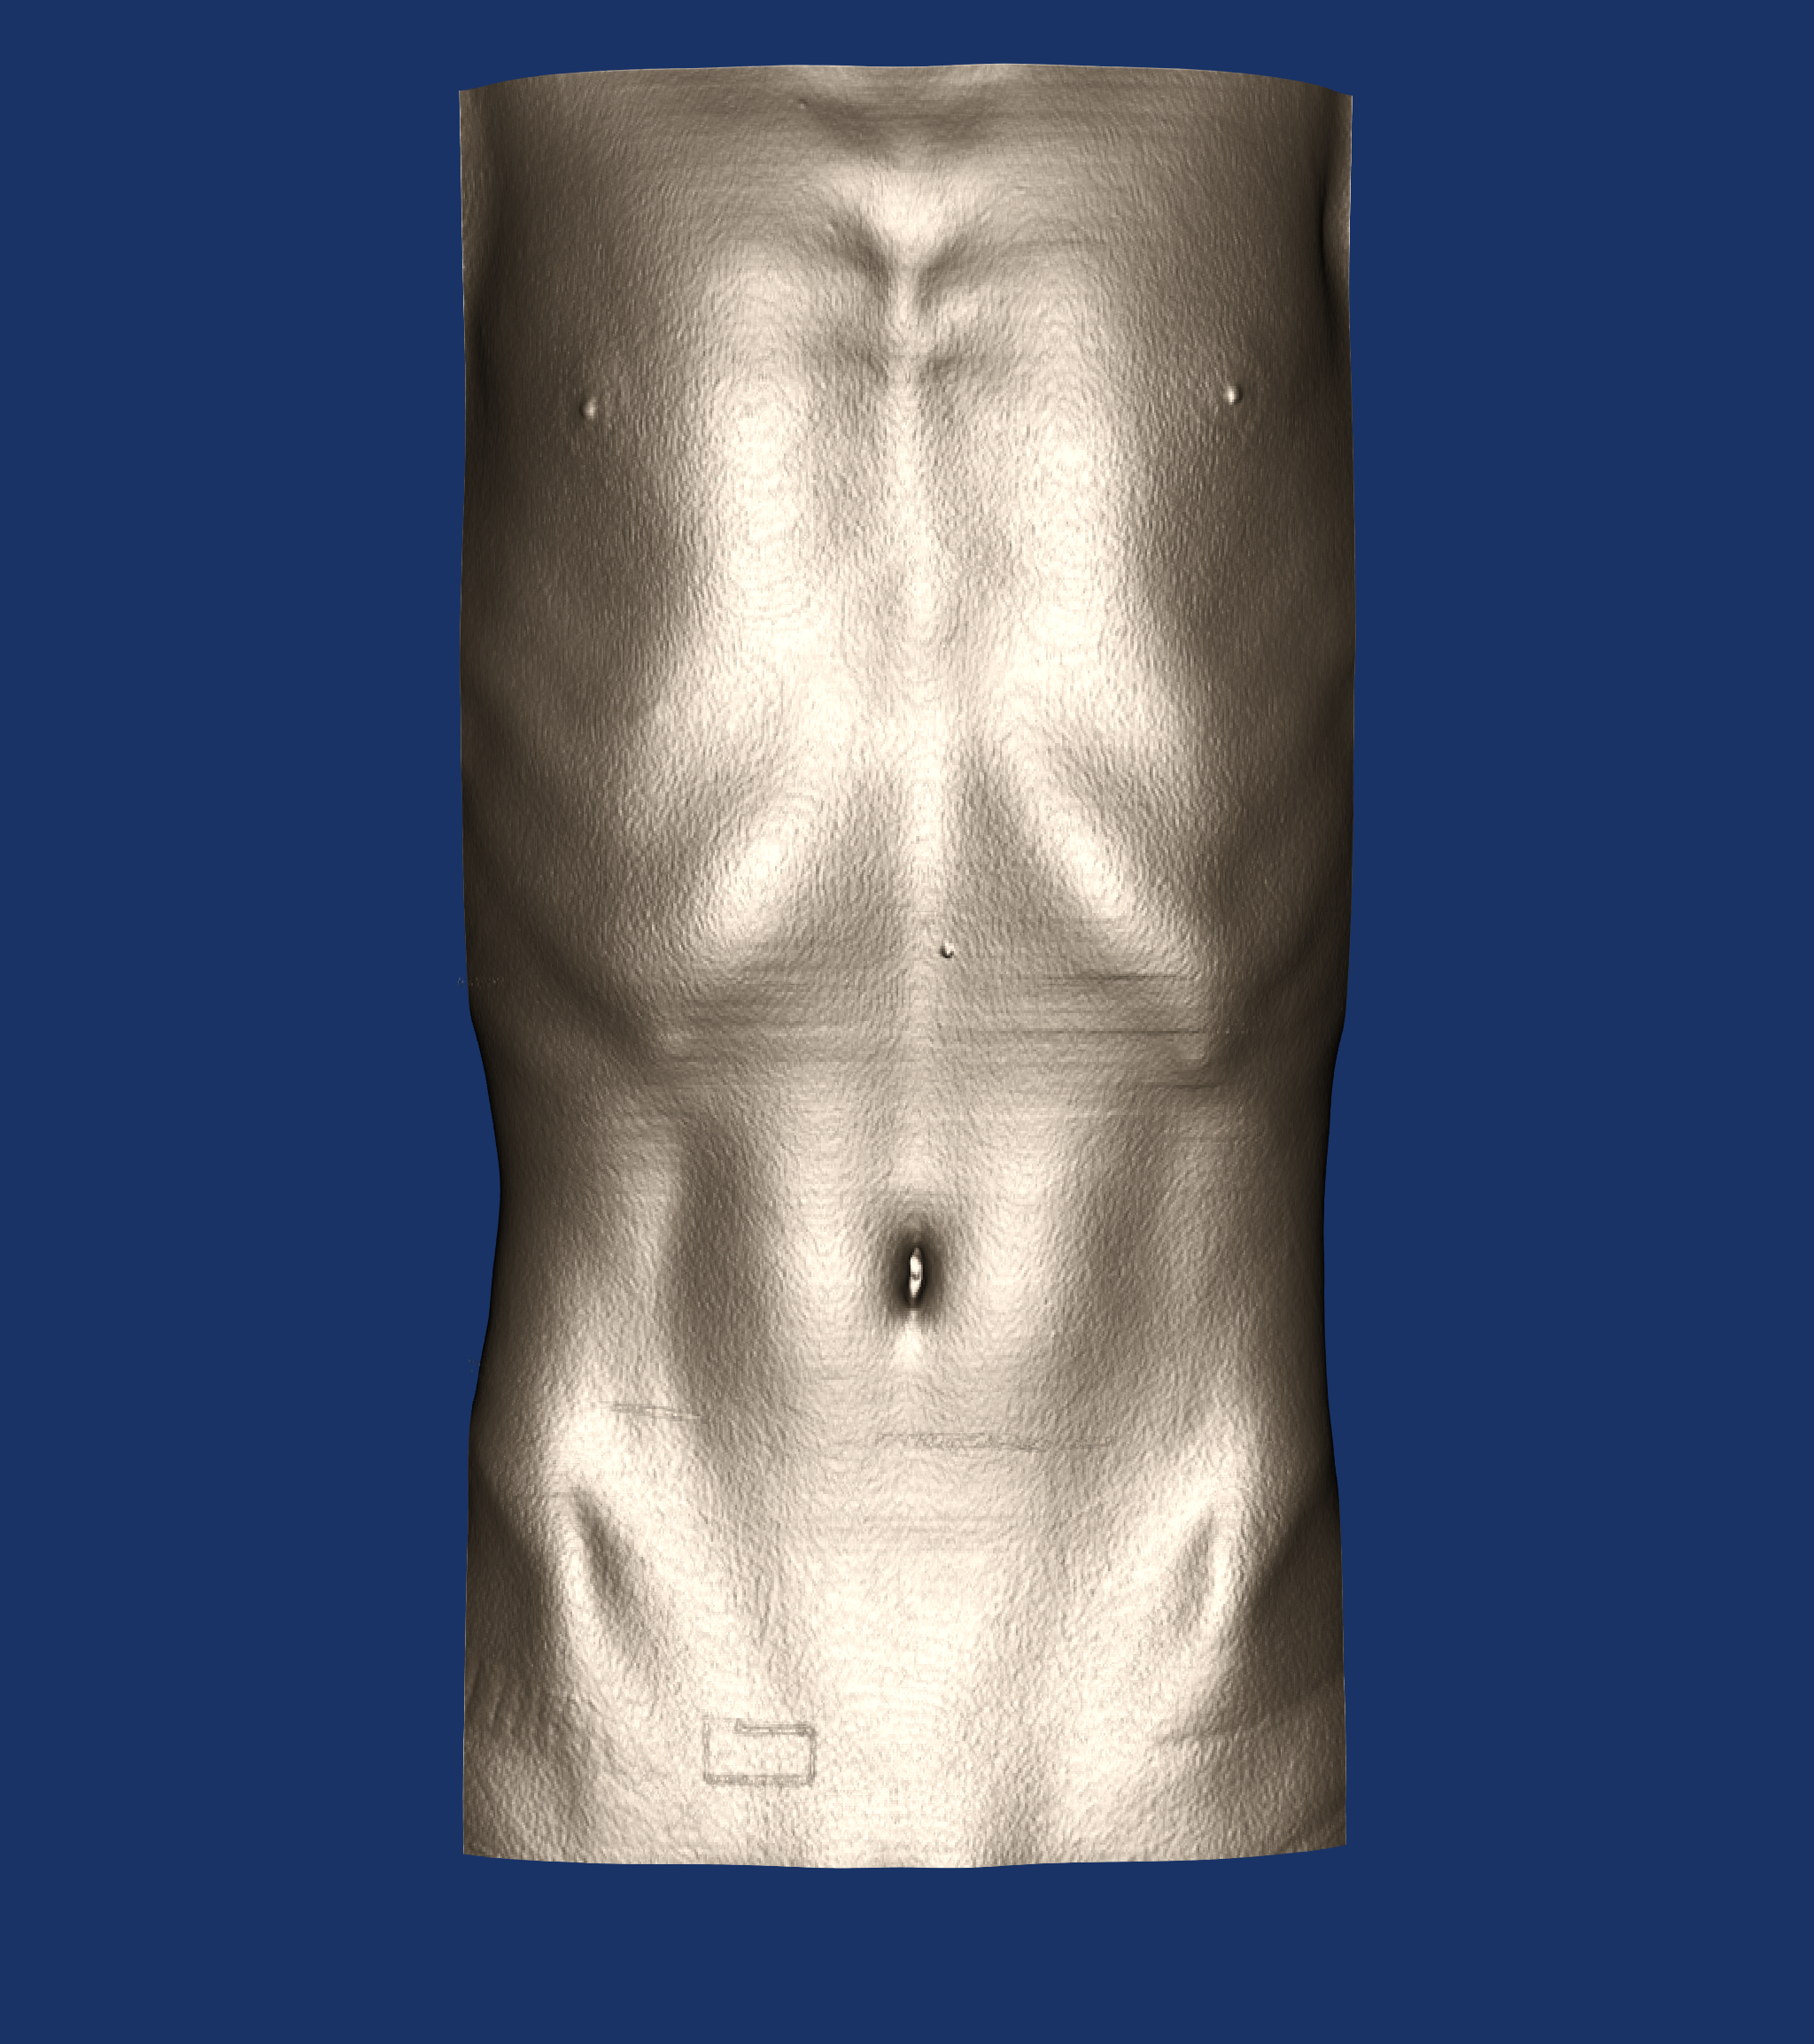
\includegraphics[width=\columnwidth]{TorsoNoGradient.png}
     \caption{Without gradient opacity function}
     \label{fig:Ng1}
   \end{subfigure}%
  \begin{subfigure}[b]{0.5\columnwidth}
    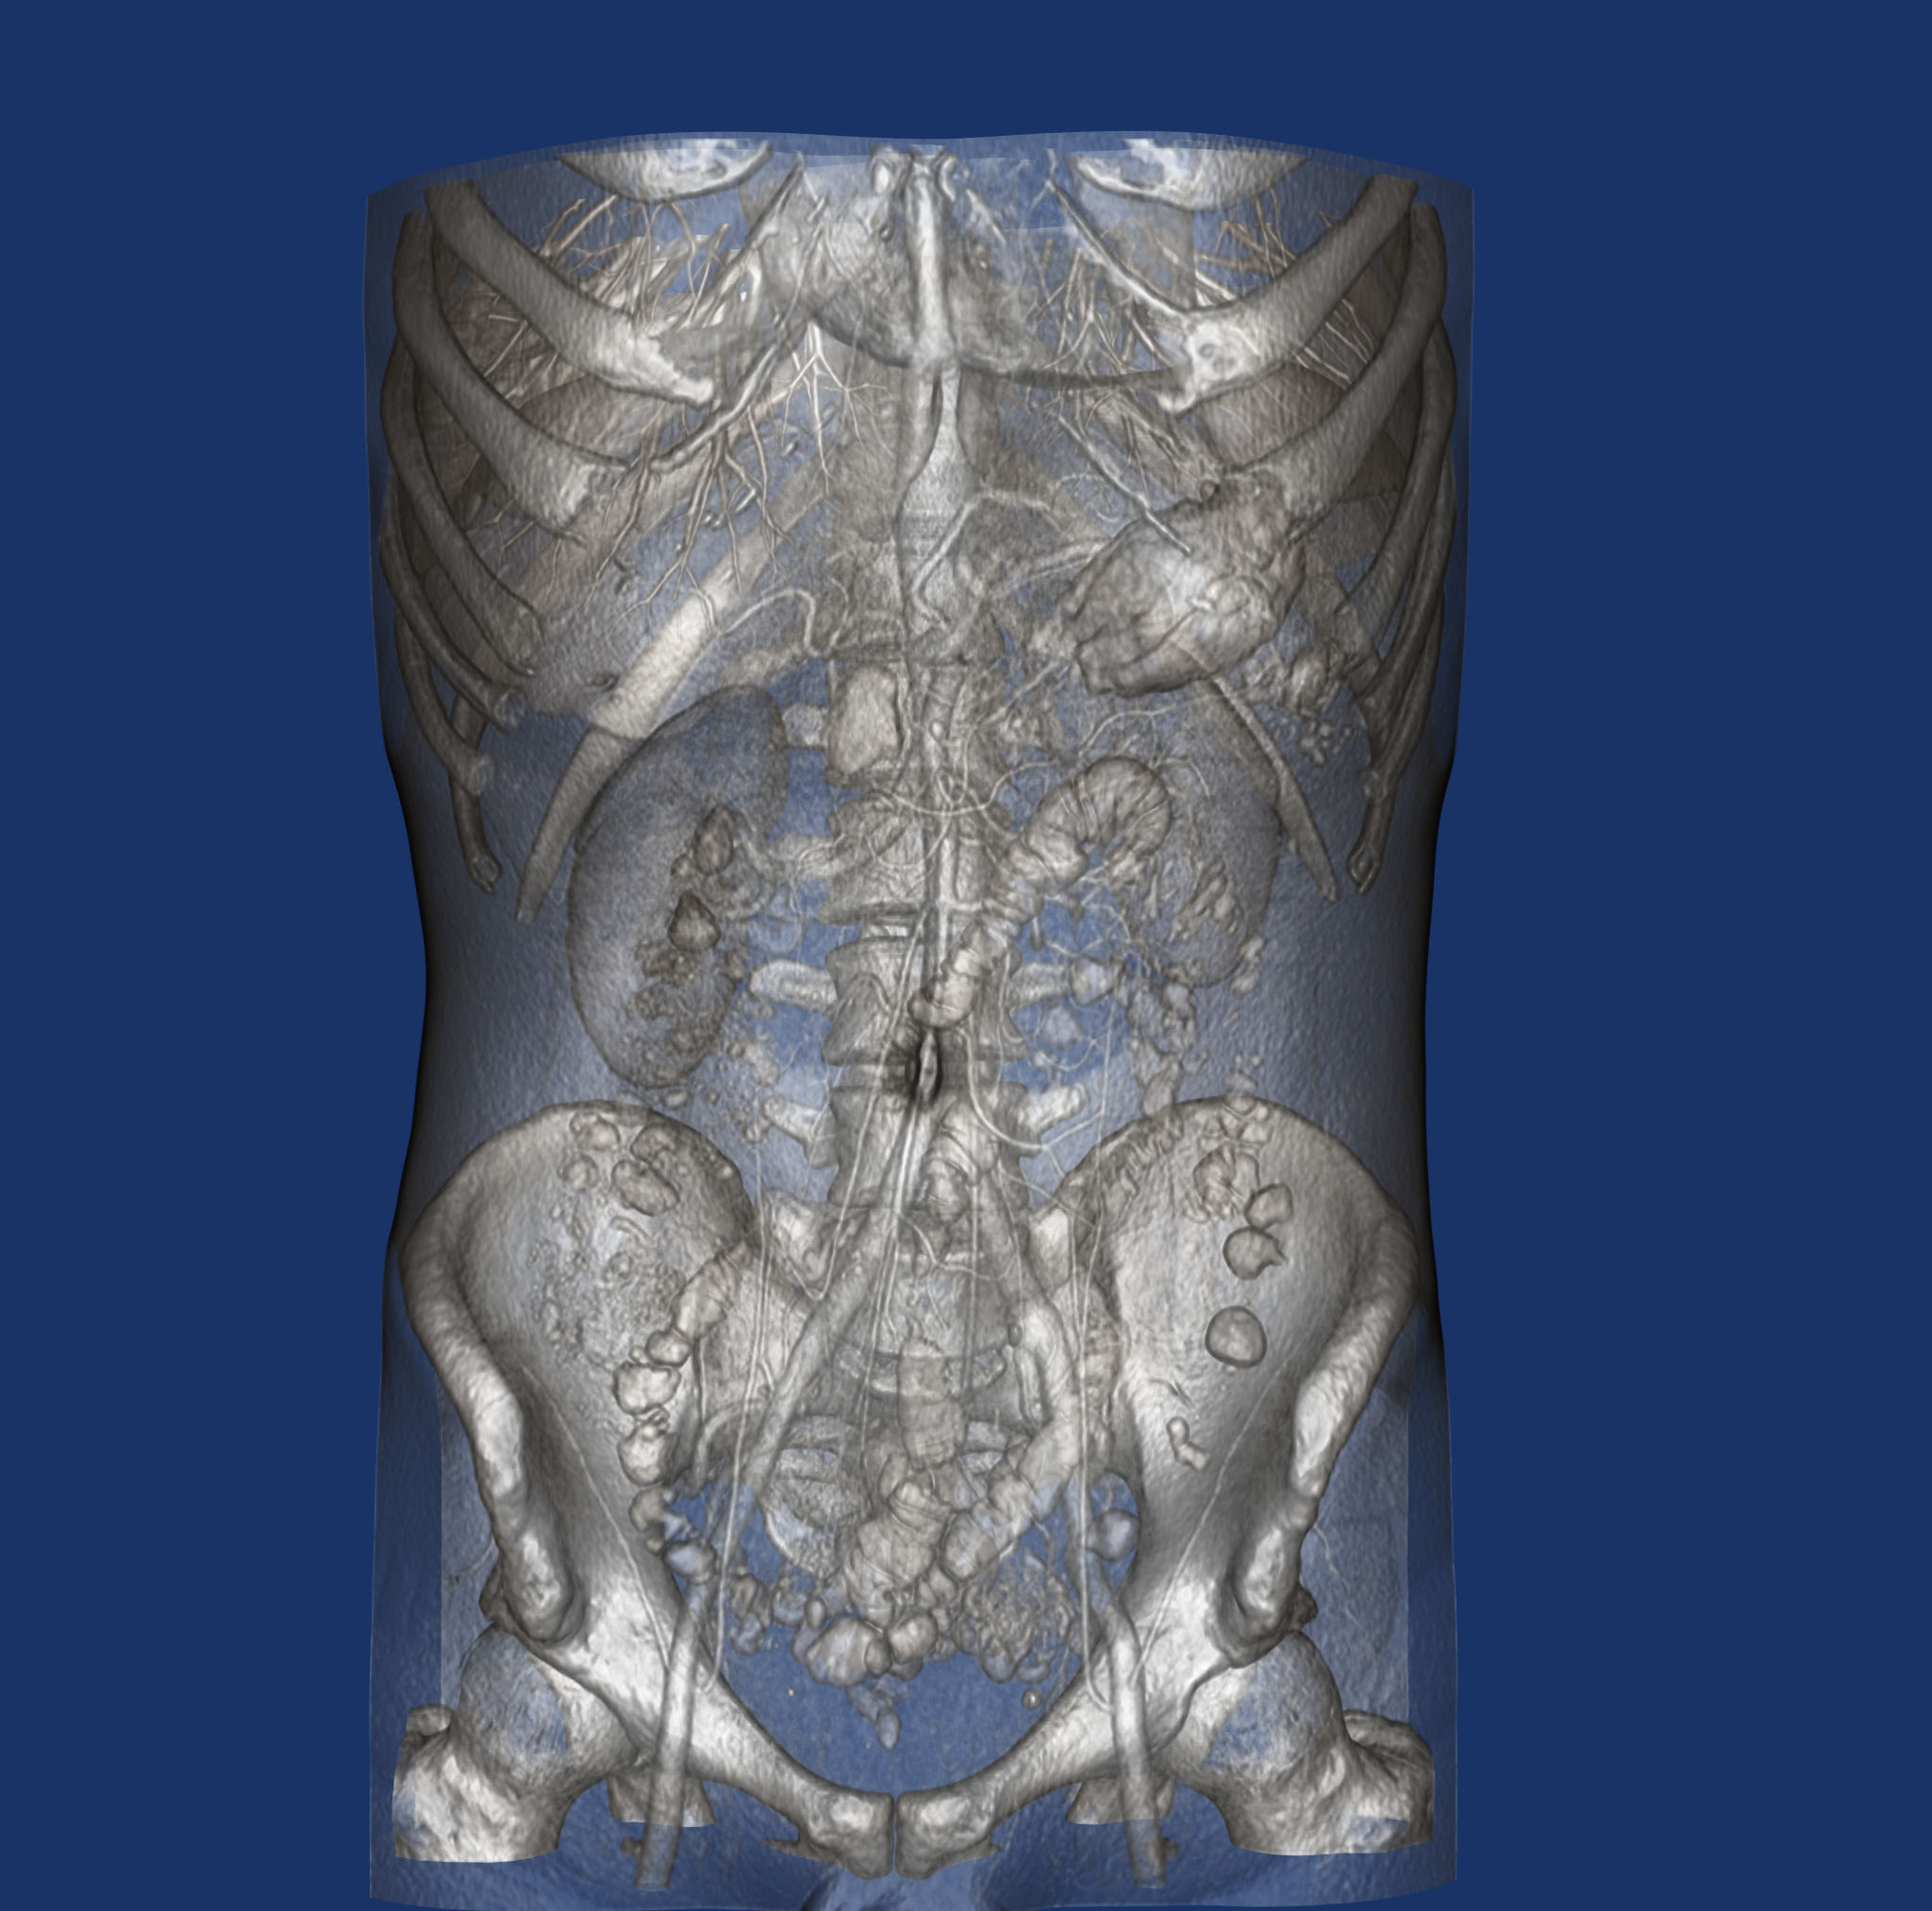
\includegraphics[width=\columnwidth]{TorsoGradient.png}
    \caption{With gradient opacity function}
    \label{fig:Ng2}
  \end{subfigure}
  \caption{Gradient magnitude based opacity modulation}
  \label{fig:gradient}
\end{figure}

\begin{figure}[htb]
  \centering
  \includegraphics[width=\columnwidth]{SMALL-PtCu-NP-Grad.png}
  \caption{Platinum-Copper (\ce{PtCu}) nanoparticle~\protect\citep{scott_electron_2012,
           miao_atomic_2016} with gradient opacity modulation enabled}
  \label{fig:ptcu-grad}
\end{figure}

\begin{figure}[htb]
  \centering
  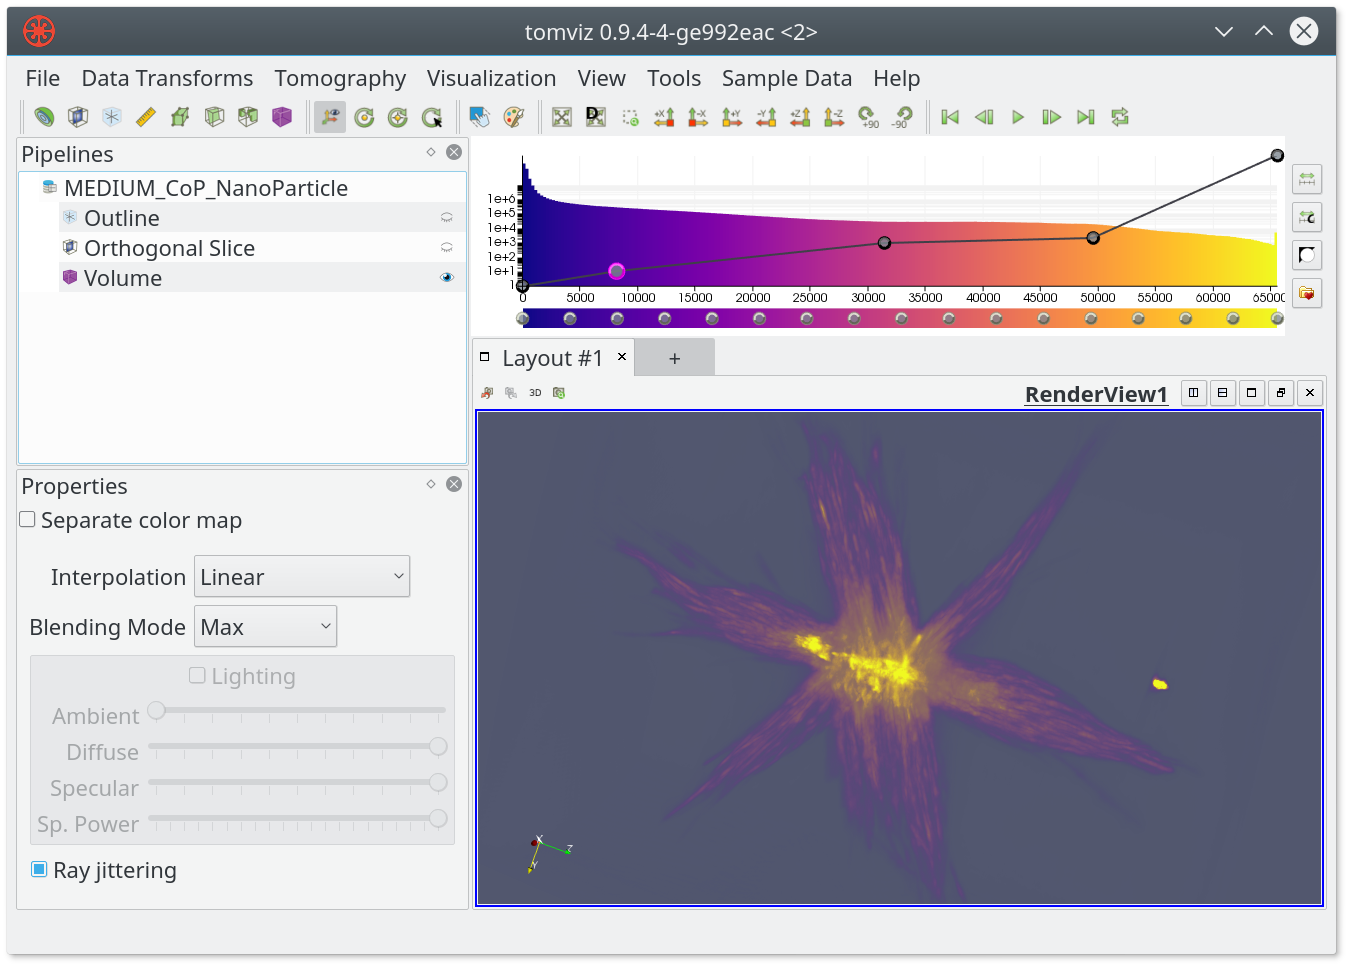
\includegraphics[width=\columnwidth]{tomviz-medium-CoP.png}
  \caption{Tomviz~\protect\citep{marcus_hanwell_tomviz_2014} rendering a
           Cobalt-Phosphorous (\ce{Co2P})
           nanoparticle~\protect\citep{levin_nanomaterial_2016}}
  \label{fig:tomviz-cop}
\end{figure}

\begin{figure}[htb]
  \centering
  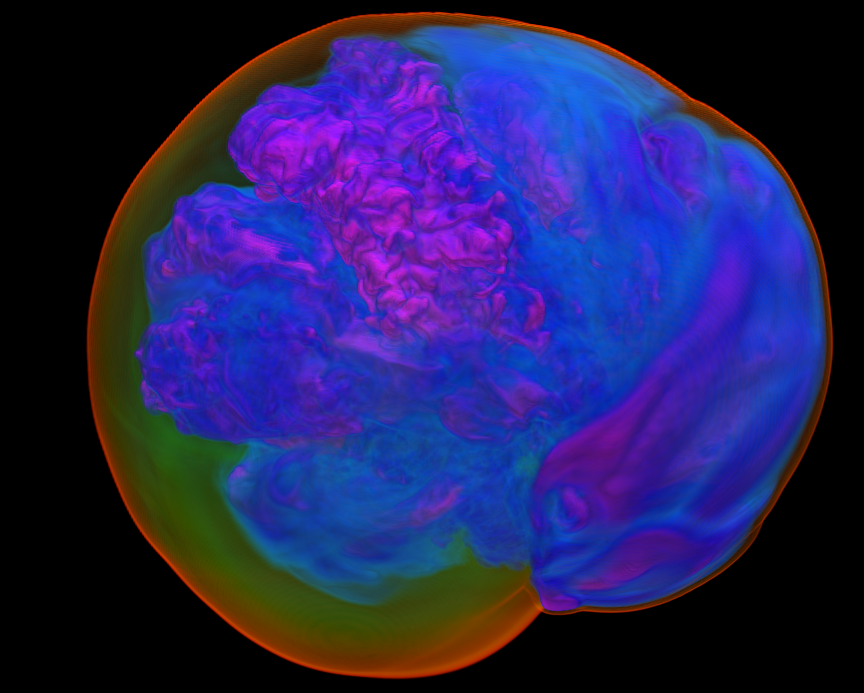
\includegraphics[width=\columnwidth]{supernova-simulation.png}
  \caption{Rendering a single timestep output of the supernova modeling
  simulation~\protect\citep{blondin_pulsar_2007}}
  \label{fig:supernova}
\end{figure}

\begin{figure}[htb]
  \centering
  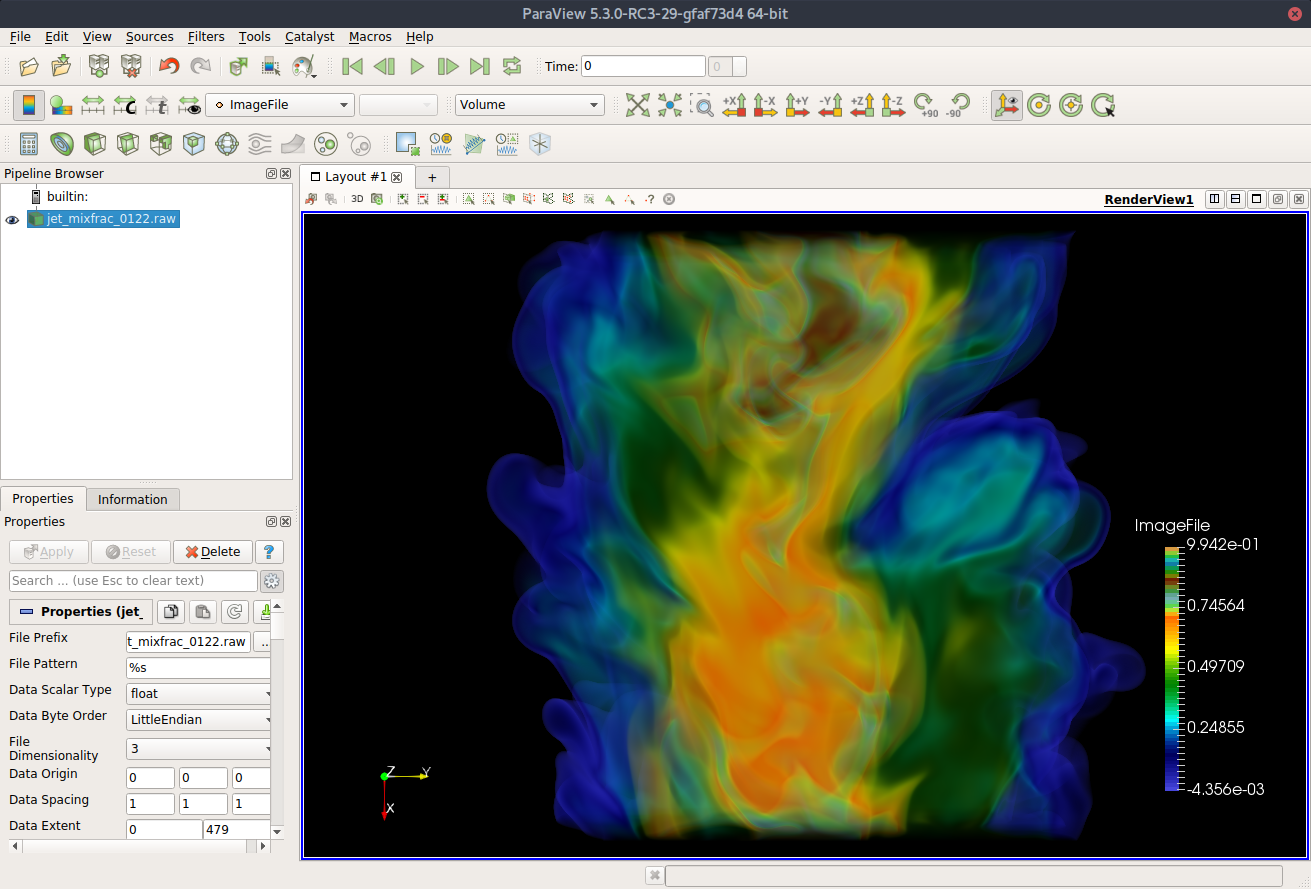
\includegraphics[width=\columnwidth]{paraview-turbulent-combustion-simulation.png}
  \caption{ParaView~\protect\citep{ahrens_paraview:_2005, ayachit_paraview_2015,
  ayachit_paraview_2015-1} rendering a single time step of a simulation of
  temporally-evolving plane jet
  flames~\protect\citep{hiroshi_akiba_visualizing_2007}}
  \label{fig:paraview-turbulent-combustion}
\end{figure}

\subsection{Performance benchmarks}
\label{performance-benchmarks}
As part of the modernization effort, we obtained several performance metrics
from sample systems with with differing specifications of hardware graphics;
ranging from on-board Intel Graphics to dedicated GPUs. The code used to
benchmark is located within the VTK code repository under
\texttt{Utilities/Benchmarks/}. The results of the
benchmark are shown in~\Autoref{fig:perf-bench}.

\begin{figure}[htbp]
  \centering
  \begin{tikzpicture}
    \begin{axis}[
      width = \linewidth,
      xlabel=Number of voxels in data (x 1 Million),
      xmode=log,
      ylabel=Frames per second,
      grid=both,
      grid style={line width=.1pt, draw=gray!10}
      ]
      \addplot[color={rgb:red,228;green,26;blue,28},mark=*] file {data/k5200.data};
      \label{plot_k52}
      \addplot[color={rgb:red,55;green,126;blue,184},mark=*] file {data/k5200_shaded.data};
      \label{plot_k52_s}
      \addplot[color={rgb:red,77;blue,175;green,74},mark=x] file {data/amdD300.data};
      \label{plot_a3}
      \addplot[color={rgb:red,152;blue,78;green,163},mark=x] file {data/amdD300_shaded.data};
      \label{plot_a3_s}
      \addplot[color={rgb:red,255;blue,127;green,0},mark=triangle*] file {data/quadro2000.data};
      \label{plot_q20}
      \addplot[color={rgb:red,255;blue,255;green,51},mark=triangle*] file {data/quadro2000_shaded.data};
      \label{plot_q20_s}
    \end{axis}
    %legend
    \node [draw,fill=white] at (rel axis cs: 0.4,0.9) {
      \shortstack[l]{
        \tiny{\textbf{Without Shading}} \\
        \ref{plot_k52} \tiny{NVIDIA Quadro K5200} \\
        \ref{plot_a3} \tiny{AMD FirePro D300}\\
        \ref{plot_q20} \tiny{NVIDIA Quadro 2000}}};
    \node [draw,fill=white] at (rel axis cs: 0.4,0.65) {
      \shortstack[l]{
        \tiny{\textbf{With Shading}} \\
        \ref{plot_k52_s} \tiny{NVIDIA Quadro K5200}\\
        \ref{plot_a3_s} \tiny{AMD FirePro D300}\\
        \ref{plot_q20_s} \tiny{NVIDIA Quadro 2000}}};
  \end{tikzpicture}
  \caption{Performance benchmarks}
  \label{fig:perf-bench}
\end{figure}
